% Source: Graph_ML/DFT_Graph_Convolution/dft_graph_convolution.tex
\begin{notechapter}
% ---- chapter-local definitions ----
\definecolor{codegreen}{rgb}{0,0.6,0}
\definecolor{codegray}{rgb}{0.5,0.5,0.5}
\definecolor{codepurple}{rgb}{0.58,0,0.82}
\definecolor{backcolour}{rgb}{0.97,0.97,0.97}
\lstdefinestyle{pythonstyle}{
    backgroundcolor=\color{backcolour},
    commentstyle=\color{codegreen},
    keywordstyle=\color{blue},
    numberstyle=\tiny\color{codegray},
    stringstyle=\color{codepurple},
    basicstyle=\ttfamily\small,
    breakatwhitespace=false,
    breaklines=true,
    captionpos=b,
    keepspaces=true,
    numbers=none,
    numbersep=5pt,
    showspaces=false,
    showstringspaces=false,
    showtabs=false,
    tabsize=4,
    frame=single,
    framerule=0.5pt,
    rulecolor=\color{gray!50},
    xleftmargin=3pt,
    xrightmargin=3pt,
}
\forgetcs\R\newcommand{\R}{\mathbb{R}}
\forgetcs\Z\newcommand{\Z}{\mathbb{Z}}
\forgetcs\C\newcommand{\C}{\mathbb{C}}
\forgetcs\N\newcommand{\N}{\mathbb{N}}
% -----------------------------------
\chapter{From the DFT to Graph Neural Networks}\label{ch:dft-to-gnn}
\chaptersubtitle{Spectral and spatial methods}

\begin{abstract}
This document develops a unified understanding of signal processing 
and neural networks on graphs. We begin by showing that the Discrete 
Fourier Transform (DFT) basis emerges naturally as the eigenvectors 
of the circular graph Laplacian---illuminating \emph{why} Fourier 
analysis works. We then generalize to arbitrary graphs via the Graph 
Fourier Transform and spectral convolution, which underpin Graph 
Convolutional Networks (GCNs). However, spectral methods have 
fundamental limitations: they require undirected graphs and expensive 
eigendecomposition. This motivates \emph{message passing}, a more 
general spatial framework that encompasses spectral methods as a 
special case. We show how this hierarchy---from classical Fourier 
analysis to modern Graph Neural Networks---reflects a progression 
from highly structured domains (the circle) to fully general graphs.
\end{abstract}

%==========================================================================
\section{Introduction: The Big Picture}
%==========================================================================

\subsection{Why This Perspective Matters}

Most introductions to the Discrete Fourier Transform present it as a 
computational tool: a way to decompose signals into sinusoids. While 
correct, this view obscures a deeper truth:

\begin{center}
\fbox{\parbox{0.85\textwidth}{
\textbf{The DFT is not an arbitrary construction.} It is the unique 
``natural'' frequency analysis for signals on a circle---forced by the 
symmetry of equally-spaced points.
}}
\end{center}

Understanding this perspective is valuable for two reasons:

\begin{enumerate}
\item It explains \emph{why} the DFT works, not just \emph{how} to 
      compute it.
\item It generalizes beautifully to \emph{any} graph structure, 
      providing the theoretical foundation for Graph Neural Networks.
\end{enumerate}

\subsection{Roadmap}

We proceed as follows:

\begin{enumerate}
\item \textbf{Part I: The Circular Graph and the DFT} (Sections 2--5)
\begin{itemize}
    \item We introduce signals on graphs and the graph Laplacian
    \item We discover that the Laplacian's eigenvectors on a circular 
          graph are exactly the DFT basis
    \item We prove the convolution theorem from this perspective
\end{itemize}

\item \textbf{Part II: Generalization to Arbitrary Graphs} 
      (Sections 6--8)
\begin{itemize}
    \item We define the Graph Fourier Transform for any graph
    \item We define spectral graph convolution
    \item We connect to Graph Convolutional Networks
\end{itemize}

\item \textbf{Part III: Limitations and Beyond} (Sections 9--10)
\begin{itemize}
    \item We examine the limitations of spectral methods (directed graphs, 
          lack of symmetry, computational cost)
    \item We introduce message passing as the general framework
    \item We show that spectral convolution is a special case of message 
          passing
\end{itemize}
\end{enumerate}

The appendix provides a detailed proof of why translation invariance 
forces complex exponentials as eigenfunctions.

%==========================================================================
\section{Signals on Graphs: The Foundation}
%==========================================================================

\subsection{What is a Signal on a Graph?}

A \textbf{graph} $G = (V, E)$ consists of a set of nodes (vertices) 
$V = \{0, 1, \ldots, N-1\}$ and edges $E$ connecting them. A 
\textbf{signal on a graph} assigns a value to each node:

\begin{equation}
\mathbf{x} = (x_0, x_1, \ldots, x_{N-1})^T \in \R^N
\end{equation}

\begin{figure}[H]
\centering
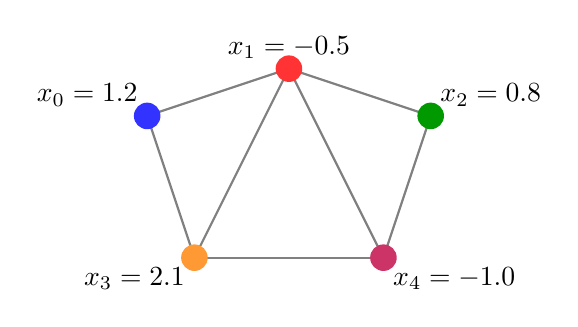
\begin{tikzpicture}[scale=1.2]
    \coordinate (A) at (0, 2);
    \coordinate (B) at (1.5, 2.5);
    \coordinate (C) at (3, 2);
    \coordinate (D) at (0.5, 0.5);
    \coordinate (E) at (2.5, 0.5);
    
    \draw[thick, gray] (A) -- (B) -- (C);
    \draw[thick, gray] (A) -- (D);
    \draw[thick, gray] (B) -- (D);
    \draw[thick, gray] (B) -- (E);
    \draw[thick, gray] (C) -- (E);
    \draw[thick, gray] (D) -- (E);
    
    \fill[blue!80] (A) circle (4pt);
    \fill[red!80] (B) circle (4pt);
    \fill[green!60!black] (C) circle (4pt);
    \fill[orange!80] (D) circle (4pt);
    \fill[purple!80] (E) circle (4pt);
    
    \node[above left] at (A) {$x_0 = 1.2$};
    \node[above] at (B) {$x_1 = -0.5$};
    \node[above right] at (C) {$x_2 = 0.8$};
    \node[below left] at (D) {$x_3 = 2.1$};
    \node[below right] at (E) {$x_4 = -1.0$};
\end{tikzpicture}
\caption{A signal on a graph with 5 nodes. Each node carries a real 
         value.}
\end{figure}

\begin{example}[Practical Examples]
\begin{itemize}
\item \textbf{Social network}: Nodes are people, edges are friendships, 
      signal is each person's age or income.
\item \textbf{Molecule}: Nodes are atoms, edges are bonds, signal is 
      atomic charge.
\item \textbf{Sensor network}: Nodes are sensors, edges connect nearby 
      sensors, signal is temperature reading.
\item \textbf{Image pixel grid}: Nodes are pixels, edges connect 
      adjacent pixels, signal is intensity.
\end{itemize}
\end{example}

\subsection{The Adjacency Matrix}

The structure of a graph is encoded in its \textbf{adjacency matrix} 
$A \in \R^{N \times N}$:

\begin{equation}
A_{ij} = \begin{cases}
a_{ij} > 0 & \text{if there is an edge from } i \text{ to } j \\
0 & \text{otherwise}
\end{cases}
\end{equation}

For unweighted graphs, $a_{ij} = 1$ when an edge exists. For undirected 
graphs, $A$ is symmetric: $A_{ij} = A_{ji}$.

\begin{remark}[Notation]
We use $A$ for the adjacency matrix throughout this document. Some 
texts use $W$ (for "weights"), but we reserve $W$ for learnable weight 
matrices in neural networks (Section~8 onwards).
\end{remark}

\subsection{The Degree Matrix and Graph Laplacian}

\begin{definition}[Degree Matrix]
The \textbf{degree} of node $i$ is the sum of edge weights connected 
to it:
\begin{equation}
d_i = \sum_{j=0}^{N-1} A_{ij}
\end{equation}
The \textbf{degree matrix} $D$ is diagonal with $D_{ii} = d_i$.
\end{definition}

\begin{definition}[Graph Laplacian]
The \textbf{(unnormalized) graph Laplacian} is:
\begin{equation}
L = D - A
\end{equation}
\end{definition}

\begin{theorem}[Properties of the Laplacian]
\label{dft-to-gnn:thm:laplacian-properties}
For an undirected graph with non-negative edge weights:
\begin{enumerate}[label=(\alph*)]
\item $L$ is symmetric and positive semi-definite.
\item All eigenvalues are non-negative: 
      $0 = \lambda_0 \leq \lambda_1 \leq \cdots \leq \lambda_{N-1}$.
\item The smallest eigenvalue $\lambda_0 = 0$ always exists, with 
      eigenvector $\mathbf{1} = (1, 1, \ldots, 1)^T$.
\item The multiplicity of $\lambda = 0$ equals the number of connected 
      components.
\end{enumerate}
\end{theorem}

\subsection{What Does the Laplacian Measure?}

The Laplacian measures \textbf{local variation} of a signal. If 
$\mathbf{y} = L\mathbf{x}$, then:

\begin{equation}
y_i = d_i x_i - \sum_{j \sim i} A_{ij} x_j 
    = \sum_{j \sim i} A_{ij}(x_i - x_j)
\end{equation}

where $j \sim i$ means $j$ is a neighbor of $i$.

\textbf{Interpretation}: $y_i$ measures how much $x_i$ differs from a 
weighted average of its neighbors. If $x_i$ equals the average, 
$y_i = 0$. If $x_i$ is larger than its neighbors, $y_i > 0$.

\begin{proposition}[Quadratic Form]
The quadratic form of the Laplacian measures total signal variation:
\begin{equation}
\mathbf{x}^T L \mathbf{x} = \frac{1}{2} \sum_{i,j} A_{ij}(x_i - x_j)^2
\end{equation}
\end{proposition}

This sum is small for \emph{smooth} signals (neighbors have similar 
values) and large for \emph{rough} signals (neighbors differ greatly).

%==========================================================================
\section{The Circular Graph: Where Fourier Analysis Emerges}
%==========================================================================

\subsection{Setting Up the Circular Graph}

Consider $N$ points arranged equally around a circle, each connected 
to its two immediate neighbors. Point $0$ connects to point $N-1$, 
closing the loop.

\begin{figure}[H]
\centering
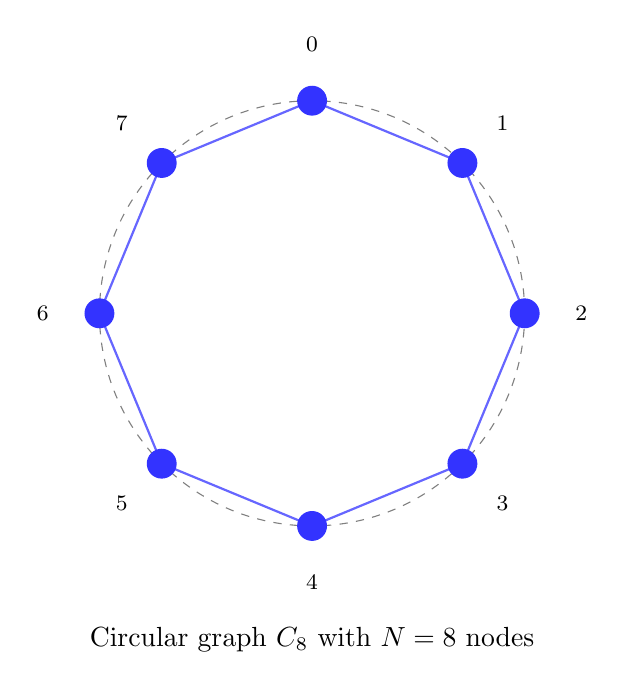
\begin{tikzpicture}[scale=1.8]
    \draw[gray, dashed] (0,0) circle (1.5);
    
    \foreach \i in {0,...,7} {
        \coordinate (n\i) at ({90 - \i*45}:1.5);
    }
    
    \draw[thick, blue!60] (n0) -- (n1);
    \draw[thick, blue!60] (n1) -- (n2);
    \draw[thick, blue!60] (n2) -- (n3);
    \draw[thick, blue!60] (n3) -- (n4);
    \draw[thick, blue!60] (n4) -- (n5);
    \draw[thick, blue!60] (n5) -- (n6);
    \draw[thick, blue!60] (n6) -- (n7);
    \draw[thick, blue!60] (n7) -- (n0);
    
    \foreach \i in {0,...,7} {
        \fill[blue!80] (n\i) circle (3pt);
        \node at ({90 - \i*45}:1.9) {\footnotesize $\i$};
    }
    
    \node at (0,-2.3) {Circular graph $C_8$ with $N = 8$ nodes};
\end{tikzpicture}
\caption{The circular graph. This structure has \textbf{perfect 
         translational symmetry}: every node ``looks the same'' as 
         every other.}
\label{dft-to-gnn:fig:circular-graph}
\end{figure}

The adjacency matrix of $C_N$ is:
\begin{equation}
W_N = \begin{pmatrix}
0 & 1 & 0 & \cdots & 0 & 1 \\
1 & 0 & 1 & \cdots & 0 & 0 \\
0 & 1 & 0 & \cdots & 0 & 0 \\
\vdots & \vdots & \vdots & \ddots & \vdots & \vdots \\
0 & 0 & 0 & \cdots & 0 & 1 \\
1 & 0 & 0 & \cdots & 1 & 0
\end{pmatrix}
\end{equation}

Since every node has degree 2, the Laplacian is:
\begin{equation}
L_N = 2I - W_N
\end{equation}

\subsection{Finding the Eigenvectors: The Key Calculation}

We seek signals $\mathbf{v}$ such that $L\mathbf{v} = \lambda\mathbf{v}$. 
The Laplacian acts on component $j$ as:
\begin{equation}
(L\mathbf{v})_j = 2v_j - v_{j-1} - v_{j+1} = \lambda v_j
\end{equation}
which rearranges to:
\begin{equation}
v_{j-1} + v_{j+1} = (2 - \lambda) v_j
\label{dft-to-gnn:eq:recurrence}
\end{equation}

This is a \textbf{linear recurrence relation}. Let's guess a solution 
of the form:
\begin{equation}
v_j = e^{i\theta j}
\end{equation}
for some angle $\theta$. Substituting into (\ref{dft-to-gnn:eq:recurrence}):
\begin{align}
e^{i\theta(j-1)} + e^{i\theta(j+1)} &= (2 - \lambda) e^{i\theta j} \\
e^{-i\theta} + e^{i\theta} &= 2 - \lambda \\
2\cos\theta &= 2 - \lambda
\end{align}

So $\lambda = 2 - 2\cos\theta = 2(1 - \cos\theta)$.

But we also need \textbf{periodicity}: the signal must satisfy 
$v_N = v_0$ (we go around the whole circle and return). This requires:
\begin{equation}
e^{i\theta N} = e^{i\theta \cdot 0} = 1
\end{equation}
which means $\theta N = 2\pi k$ for some integer $k$, i.e., 
$\theta = \frac{2\pi k}{N}$.

\begin{theorem}[Eigenvectors of the Circular Graph Laplacian]
\label{dft-to-gnn:thm:circular-eigenvectors}
The eigenvectors of $L_N = 2I - W_N$ are:
\begin{equation}
\mathbf{v}_k = \frac{1}{\sqrt{N}}
\begin{pmatrix}
1 \\ e^{2\pi i k/N} \\ e^{2\pi i \cdot 2k/N} \\ \vdots \\ 
e^{2\pi i (N-1)k/N}
\end{pmatrix}, \quad k = 0, 1, \ldots, N-1
\end{equation}
with corresponding eigenvalues:
\begin{equation}
\lambda_k = 2 - 2\cos\left(\frac{2\pi k}{N}\right) 
          = 4\sin^2\left(\frac{\pi k}{N}\right)
\end{equation}
These eigenvectors are orthonormal: 
$\mathbf{v}_j^* \mathbf{v}_k = \delta_{jk}$.
\end{theorem}

\begin{figure}[H]
\centering
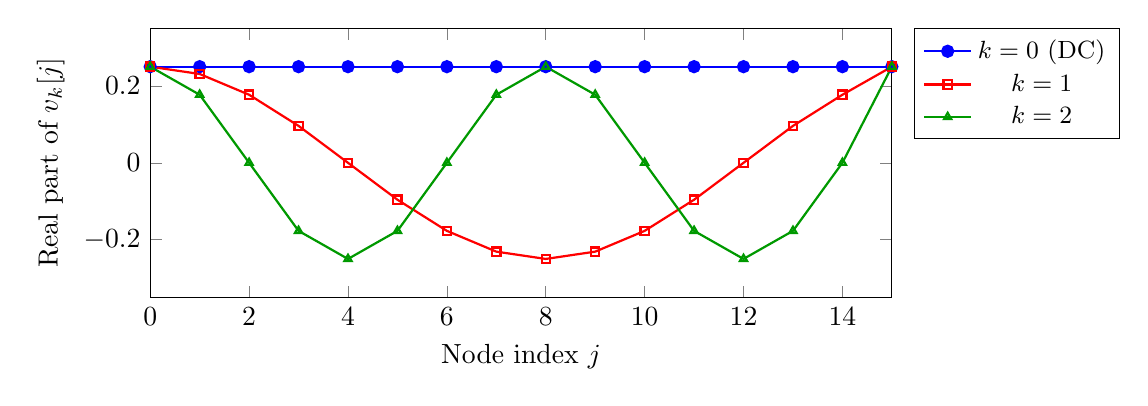
\begin{tikzpicture}
\begin{axis}[
    width=11cm, height=5cm, % Reduced width to create space for the legend
    xlabel={Node index $j$},
    ylabel={Real part of $v_k[j]$},
    xmin=0, xmax=15,
    ymin=-0.35, ymax=0.35,
    % Moves the legend outside the plotting area to the right
    legend pos=outer north east, 
    legend style={font=\small},
]
% k=0 (constant)
\addplot[thick, blue, mark=*] coordinates {
    (0,0.25) (1,0.25) (2,0.25) (3,0.25) (4,0.25) (5,0.25) (6,0.25) 
    (7,0.25) (8,0.25) (9,0.25) (10,0.25) (11,0.25) (12,0.25) 
    (13,0.25) (14,0.25) (15,0.25)
};
\addlegendentry{$k=0$ (DC)}

% k=1
\addplot[thick, red, mark=square, mark size=1.5pt] coordinates {
    (0,0.25) (1,0.231) (2,0.177) (3,0.096) (4,0) (5,-0.096) 
    (6,-0.177) (7,-0.231) (8,-0.25) (9,-0.231) (10,-0.177) 
    (11,-0.096) (12,0) (13,0.096) (14,0.177) (15,0.25)
};
\addlegendentry{$k=1$}

% k=2
\addplot[thick, green!60!black, mark=triangle, mark size=1.5pt] 
    coordinates {
    (0,0.25) (1,0.177) (2,0) (3,-0.177) (4,-0.25) (5,-0.177) 
    (6,0) (7,0.177) (8,0.25) (9,0.177) (10,0) (11,-0.177) 
    (12,-0.25) (13,-0.177) (14,0) (15,0.25)
};
\addlegendentry{$k=2$}
\end{axis}
\end{tikzpicture}

\caption{Real parts of the first three eigenvectors for $N=16$. These 
         are samples of cosine waves at frequencies $0, 1, 2$ cycles 
         around the circle.}
\end{figure}

\subsection{Interpretation: Vibration Modes}

Think of the circular graph as a ring of masses connected by springs. 
The eigenvectors represent the natural \textbf{vibration modes}:

\begin{itemize}
\item $k = 0$: All masses move together (rigid translation). 
      Eigenvalue $\lambda_0 = 0$.
\item $k = 1$: One complete wave around the ring. Low eigenvalue 
      (slow oscillation).
\item $k = N/2$ (if $N$ even): Alternating pattern $+,-,+,-,\ldots$ 
      Highest eigenvalue (fastest oscillation).
\end{itemize}

\subsection{The Punchline: These ARE the DFT Basis Vectors!}

Recall the standard DFT:
\begin{equation}
X_k = \sum_{n=0}^{N-1} x_n \, e^{-2\pi i kn/N}
\end{equation}

The $k$-th DFT coefficient is the inner product of the signal 
$\mathbf{x}$ with the vector 
$(1, e^{2\pi i k/N}, e^{2\pi i \cdot 2k/N}, \ldots)^T$---exactly our 
eigenvector $\mathbf{v}_k$ (up to conjugation and normalization)!

\begin{center}
\fbox{\parbox{0.9\textwidth}{
\textbf{Key Insight}: The DFT basis vectors are the eigenvectors of 
the circular graph Laplacian. The DFT is not an arbitrary choice---it 
is \emph{forced} by the circular symmetry of equally-spaced points.
}}
\end{center}

\begin{remark}
Why are complex exponentials the eigenvectors? This is not a 
coincidence---it is a deep consequence of \textbf{translation 
invariance}. Any operator that commutes with circular shifts must 
have complex exponentials as eigenfunctions. See 
Appendix~\ref{dft-to-gnn:app:translation-invariance} for a detailed proof.
\end{remark}

%==========================================================================
\section{The DFT as Eigendecomposition}
%==========================================================================

\subsection{Matrix Formulation}

Define the \textbf{DFT matrix} $F \in \C^{N \times N}$ with entries:
\begin{equation}
F_{kn} = e^{-2\pi i kn/N} = \omega^{kn}, 
\quad \text{where } \omega = e^{-2\pi i/N}
\end{equation}

Then the DFT is matrix multiplication:
\begin{equation}
\mathbf{X} = F \mathbf{x}
\end{equation}

\begin{example}[DFT Matrix for $N = 4$]
With $\omega = e^{-2\pi i/4} = -i$:
\[
F_4 = \begin{pmatrix}
1 & 1 & 1 & 1 \\
1 & -i & -1 & i \\
1 & -1 & 1 & -1 \\
1 & i & -1 & -i
\end{pmatrix}
\]
The columns of $F^*$ (conjugate transpose) are the eigenvectors we 
found: $(1, 1, 1, 1)$, $(1, i, -1, -i)$, $(1, -1, 1, -1)$, 
$(1, -i, -1, i)$.
\end{example}

\subsection{The DFT Diagonalizes the Circular Laplacian}

\begin{theorem}[Diagonalization]
The circular graph Laplacian is diagonalized by the (normalized) DFT 
matrix:
\begin{equation}
L_N = Q \Lambda Q^*
\end{equation}
where $Q = \frac{1}{\sqrt{N}} F^*$ has the eigenvectors as columns, 
and $\Lambda = \text{diag}(\lambda_0, \lambda_1, \ldots, \lambda_{N-1})$.
\end{theorem}

This means expressing a signal in the DFT basis is equivalent to 
expressing it in the eigenbasis of the Laplacian. The DFT coefficient 
$X_k$ measures how much of the $k$-th eigenvector (the $k$-th 
``frequency mode'') is present in the signal.

\subsection{Frequency Interpretation of Eigenvalues}

The eigenvalues $\lambda_k = 4\sin^2(\pi k/N)$ have a natural 
interpretation:

\begin{itemize}
\item $\lambda_0 = 0$: The constant signal. No variation between 
      neighbors.
\item $\lambda_k$ small: Low-frequency modes. Slow variation around 
      the circle.
\item $\lambda_k$ large: High-frequency modes. Rapid variation between 
      neighbors.
\item $\lambda_{N/2} = 4$ (for even $N$): The alternating signal 
      $(-1)^n$. Maximum variation.
\end{itemize}

\begin{figure}[H]
\centering
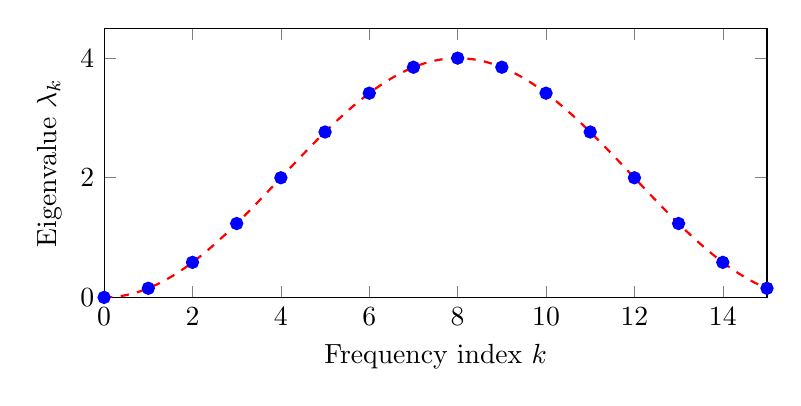
\begin{tikzpicture}
\begin{axis}[
    width=10cm, height=5cm,
    xlabel={Frequency index $k$},
    ylabel={Eigenvalue $\lambda_k$},
    xmin=0, xmax=15,
    ymin=0, ymax=4.5,
]
\addplot[thick, blue, mark=*, only marks] coordinates {
    (0, 0) (1, 0.152) (2, 0.586) (3, 1.235) (4, 2) (5, 2.765) 
    (6, 3.414) (7, 3.848) (8, 4) (9, 3.848) (10, 3.414) (11, 2.765)
    (12, 2) (13, 1.235) (14, 0.586) (15, 0.152)
};
\addplot[thick, red, dashed, samples=100, domain=0:15] 
    {4*sin(deg(pi*x/16))^2};
\end{axis}
\end{tikzpicture}
\caption{Eigenvalues $\lambda_k = 4\sin^2(\pi k/N)$ for $N=16$. Higher 
         $k$ means higher eigenvalue (more variation).}
\end{figure}

%==========================================================================
\section{Convolution and the Convolution Theorem}
%==========================================================================

\subsection{Two Types of Convolution}

It's crucial to distinguish between two different convolution operations:

\begin{definition}[Linear Convolution]
Given signals $x[n]$ (length $N$) and $h[n]$ (length $M$), their 
\textbf{linear convolution} is:
\begin{equation}
y[n] = (x * h)[n] = \sum_{m=-\infty}^{\infty} x[m] h[n-m]
\end{equation}
For finite signals with $x[n]=0$ for $n<0$ or $n\geq N$, and 
$h[n]=0$ for $n<0$ or $n\geq M$, this becomes:
\begin{equation}
y[n] = \sum_{m=0}^{N-1} x[m] h[n-m]
\end{equation}
where $h[n-m]$ is taken as 0 when $n-m$ is outside $[0, M-1]$. The 
result has length $N+M-1$.
\end{definition}

\begin{definition}[Circular Convolution]
Given signals $\mathbf{x}, \mathbf{h} \in \C^N$ both of length $N$, 
their \textbf{circular convolution} is:
\begin{equation}
y[n] = (\mathbf{x} \circledast \mathbf{h})[n] = \sum_{m=0}^{N-1} x[m] 
        h[(n-m) \mod N]
\end{equation}
The result has length $N$, with wrap-around due to the modulo operation.
\end{definition}

\begin{example}[Linear vs Circular Convolution]
Let $x = [1, 2, 3]$ and $h = [1, 1]$.
\begin{itemize}
\item \textbf{Linear convolution}: 
  \[
  y = x * h = [1\cdot1, 1\cdot1+2\cdot1, 2\cdot1+3\cdot1, 3\cdot1] 
    = [1, 3, 5, 3]
  \]
  (length $3+2-1 = 4$)
\item \textbf{Circular convolution} (pad $h$ to length 3: $[1, 1, 0]$):
  \begin{align*}
  y[0] &= x[0]h[0] + x[1]h[2] + x[2]h[1] = 1\cdot1 + 2\cdot0 + 3\cdot1 = 4 \\
  y[1] &= x[0]h[1] + x[1]h[0] + x[2]h[2] = 1\cdot1 + 2\cdot1 + 3\cdot0 = 3 \\
  y[2] &= x[0]h[2] + x[1]h[1] + x[2]h[0] = 1\cdot0 + 2\cdot1 + 3\cdot1 = 5
  \end{align*}
  So $y = x \circledast h = [4, 3, 5]$ (length 3)
\end{itemize}
Notice the circular convolution gives a different first element (4 instead of 1)
because of wrap-around: $x[1]h[2]$ uses $h[2] = h[-1 \mod 3] = h[2] = 0$.
\end{example}

\subsection{Circulant Matrices Represent Circular Convolution}

Circular convolution can be written as a matrix-vector product 
$\mathbf{y} = C_h \mathbf{x}$, where $C_h$ is a \textbf{circulant 
matrix}:

\begin{equation}
C_h = \begin{pmatrix}
h_0 & h_{N-1} & h_{N-2} & \cdots & h_1 \\
h_1 & h_0 & h_{N-1} & \cdots & h_2 \\
h_2 & h_1 & h_0 & \cdots & h_3 \\
\vdots & \vdots & \vdots & \ddots & \vdots \\
h_{N-1} & h_{N-2} & h_{N-3} & \cdots & h_0
\end{pmatrix}
\end{equation}

Each row is a cyclic shift of the previous one. The $(i,j)$ entry is 
$C_{ij} = h_{(i-j) \mod N}$.

\subsection{Circulant Matrices and the DFT}

\begin{theorem}[All Circulant Matrices Share the Same Eigenvectors]
\label{dft-to-gnn:thm:circulant-eigenvectors}
Every circulant matrix $C$ is diagonalized by the DFT matrix:
\begin{equation}
C = F^{-1} \, \text{diag}(\text{DFT}(\mathbf{c})) \, F
\end{equation}
where $\mathbf{c} = (c_0, c_1, \ldots, c_{N-1})^T$ is the first column 
of $C$.
\end{theorem}

\begin{proof}[Detailed proof]
Let $C$ be a circulant matrix with first column $\mathbf{c} = 
(c_0, c_1, \ldots, c_{N-1})^T$. The $(i,j)$ entry is:
\[
C_{ij} = c_{(i-j) \mod N}
\]

Let $\mathbf{v}_k$ be the $k$-th DFT basis vector (normalized):
\[
\mathbf{v}_k = \frac{1}{\sqrt{N}} 
\begin{pmatrix}
1 \\ e^{2\pi i k/N} \\ e^{4\pi i k/N} \\ \vdots \\ e^{2\pi i (N-1)k/N}
\end{pmatrix}
\]

Compute $(C\mathbf{v}_k)[n]$:
\begin{align*}
(C\mathbf{v}_k)[n] 
    &= \sum_{m=0}^{N-1} C_{nm} \mathbf{v}_k[m] \\
    &= \sum_{m=0}^{N-1} c_{(n-m) \mod N} \cdot \frac{1}{\sqrt{N}} 
       e^{2\pi i mk/N}
\end{align*}

Change variable: $\ell = (n-m) \mod N$, so $m = (n-\ell) \mod N$, and 
$e^{2\pi i mk/N} = e^{2\pi i (n-\ell)k/N} = e^{2\pi i nk/N} 
\cdot e^{-2\pi i \ell k/N}$:

\begin{align*}
(C\mathbf{v}_k)[n] 
    &= \frac{1}{\sqrt{N}} \sum_{\ell=0}^{N-1} c_\ell 
       \left( e^{2\pi i nk/N} \cdot e^{-2\pi i \ell k/N} \right) \\
    &= \frac{1}{\sqrt{N}} e^{2\pi i nk/N} 
       \sum_{\ell=0}^{N-1} c_\ell \, e^{-2\pi i \ell k/N} \\
    &= \mathbf{v}_k[n] \cdot \underbrace{\sum_{\ell=0}^{N-1} c_\ell 
       e^{-2\pi i \ell k/N}}_{\text{DFT}(\mathbf{c})_k}
\end{align*}

Thus $C\mathbf{v}_k = \text{DFT}(\mathbf{c})_k \cdot \mathbf{v}_k$, 
proving $\mathbf{v}_k$ is an eigenvector with eigenvalue 
$\text{DFT}(\mathbf{c})_k$. This holds for all circulant matrices $C$
using the same eigenvectors $\mathbf{v}_k$.
\end{proof}

\textbf{Key insight}: The circular graph Laplacian $L = 2I - W$ is 
itself a circulant matrix. Theorem~\ref{dft-to-gnn:thm:circulant-eigenvectors} 
tells us that \emph{all} circulant matrices---including all 
\textbf{circular convolution} operators---share the same eigenvectors: 
the DFT basis.

\subsection{The Convolution Theorem for Circular Convolution}

\begin{theorem}[Convolution Theorem for Circular Convolution]
\label{dft-to-gnn:thm:convolution-circular}
Let $\mathbf{X} = \text{DFT}(\mathbf{x})$, 
$\mathbf{H} = \text{DFT}(\mathbf{h})$, and 
$\mathbf{Y} = \text{DFT}(\mathbf{x} \circledast \mathbf{h})$, where 
$\circledast$ denotes \textbf{circular convolution}. Then:
\begin{equation}
Y_k = X_k \cdot H_k \quad \text{for all } k
\end{equation}
\textbf{Circular convolution in the time domain equals pointwise 
multiplication in the frequency domain.}
\end{theorem}

\begin{proof}
Since circular convolution corresponds to multiplication by a circulant 
matrix $\mathbf{y} = C_h \mathbf{x}$, and we just showed $C_h$ is 
diagonalized by the DFT:
\begin{equation}
\mathbf{Y} = F\mathbf{y} = F C_h \mathbf{x} 
           = F C_h F^{-1} \cdot F\mathbf{x} 
           = \text{diag}(\mathbf{H}) \cdot \mathbf{X}
\end{equation}
which is componentwise multiplication.
\end{proof}

\subsection{Linear Convolution via DFT with Zero Padding}

The DFT naturally gives us \textbf{circular convolution}, but we often 
want \textbf{linear convolution}. The solution is \textbf{zero padding}:

\begin{theorem}[Linear Convolution via DFT]
Given $x[n]$ (length $N$) and $h[n]$ (length $M$), let $L \geq N+M-1$. 
Define zero-padded versions:
\begin{align*}
x_{\text{pad}}[n] &= \begin{cases}
x[n] & 0 \leq n < N \\
0 & N \leq n < L
\end{cases} \\
h_{\text{pad}}[n] &= \begin{cases}
h[n] & 0 \leq n < M \\
0 & M \leq n < L
\end{cases}
\end{align*}
Then the linear convolution $y = x * h$ can be computed as:
\begin{equation}
y[n] = \text{IDFT}\left(\text{DFT}(x_{\text{pad}}) \odot 
       \text{DFT}(h_{\text{pad}})\right)[n]
\end{equation}
for $0 \leq n \leq N+M-2$, where $\odot$ denotes element-wise 
multiplication.
\end{theorem}

\begin{proof}[Proof sketch]
With sufficient zero-padding ($L \geq N+M-1$), the circular convolution 
of the padded signals equals the linear convolution of the original 
signals, because the zeros prevent wrap-around interference between 
periods in the DFT's implicit periodic extension.
\end{proof}

\subsection{Detailed Example: Computing Linear Convolution via DFT}

Let's work through a complete example to see exactly how zero-padding allows us to compute 
linear convolution using the DFT.

\begin{example}[Computing Linear Convolution via DFT - Detailed]
Let $x = [1, 2, 3]$ ($N=3$) and $h = [1, 1]$ ($M=2$). The linear convolution should yield:
\[
y = x * h = [1, 3, 5, 3]
\]
with length $L_y = N + M - 1 = 3 + 2 - 1 = 4$.

Indeed, the convolution is defined by the formula:
\[
y[n] = \sum_{k=-\infty}^{\infty} x[k]h[n-k]
\]
Therefore:
\begin{align*}
    y[0] &= x[0]h[0] = 1 \cdot 1 = 1 \\
    y[1] &= x[0]h[1] + x[1]h[0] = (1 \cdot 1) + (2 \cdot 1) = 3 \\
    y[2] &= x[1]h[1] + x[2]h[0] = (2 \cdot 1) + (3 \cdot 1) = 5 \\
    y[3] &= x[2]h[1] = 3 \cdot 1 = 3
\end{align*}


\vspace{0.3cm}
\textbf{Step 1: Zero-padding}

We need to pad both signals to length $L \geq N + M - 1 = 4$. Let's choose $L = 4$:
\begin{align*}
x_{\text{pad}} &= [1, 2, 3, 0] \\
h_{\text{pad}} &= [1, 1, 0, 0]
\end{align*}

\vspace{0.3cm}
\textbf{Step 2: Compute DFTs}

For $L=4$, the DFT matrix uses $\omega = e^{-2\pi i/4} = e^{-\pi i/2} = -i$.

The DFT matrix is:
\[
F_4 = \begin{pmatrix}
1 & 1 & 1 & 1 \\
1 & -i & -1 & i \\
1 & -1 & 1 & -1 \\
1 & i & -1 & -i
\end{pmatrix}
\]

Compute $\mathbf{X} = F_4 x_{\text{pad}}$:
\begin{align*}
X[0] &= 1 + 2 + 3 + 0 = 6 \\
X[1] &= 1 + 2(-i) + 3(-1) + 0(i) = 1 - 2i - 3 = -2 - 2i \\
X[2] &= 1 + 2(-1) + 3(1) + 0(-1) = 1 - 2 + 3 = 2 \\
X[3] &= 1 + 2(i) + 3(-1) + 0(-i) = 1 + 2i - 3 = -2 + 2i
\end{align*}
So $\mathbf{X} = [6, -2-2i, 2, -2+2i]$.

Compute $\mathbf{H} = F_4 h_{\text{pad}}$:
\begin{align*}
H[0] &= 1 + 1 + 0 + 0 = 2 \\
H[1] &= 1 + 1(-i) + 0(-1) + 0(i) = 1 - i \\
H[2] &= 1 + 1(-1) + 0(1) + 0(-1) = 1 - 1 = 0 \\
H[3] &= 1 + 1(i) + 0(-1) + 0(-i) = 1 + i
\end{align*}
So $\mathbf{H} = [2, 1-i, 0, 1+i]$.

\vspace{0.3cm}
\textbf{Step 3: Multiply in frequency domain}

Element-wise multiplication: $Y[k] = X[k] \cdot H[k]$
\begin{align*}
Y[0] &= 6 \times 2 = 12 \\
Y[1] &= (-2-2i) \times (1-i) = (-2-2i)(1-i) = -2(1-i) -2i(1-i) \\
     &= -2 + 2i - 2i + 2i^2 = -2 - 2 = -4 \quad (\text{since } i^2 = -1) \\
Y[2] &= 2 \times 0 = 0 \\
Y[3] &= (-2+2i) \times (1+i) = (-2+2i)(1+i) = -2(1+i) + 2i(1+i) \\
     &= -2 - 2i + 2i + 2i^2 = -2 - 2 = -4
\end{align*}
So $\mathbf{Y} = [12, -4, 0, -4]$.

\vspace{0.3cm}
\textbf{Step 4: Inverse DFT}

The inverse DFT matrix is $F_4^{-1} = \frac{1}{4} F_4^*$ (conjugate transpose).

Compute $\mathbf{y} = F_4^{-1} \mathbf{Y} = \frac{1}{4} F_4^* \mathbf{Y}$:
\[
F_4^* = \begin{pmatrix}
1 & 1 & 1 & 1 \\
1 & i & -1 & -i \\
1 & -1 & 1 & -1 \\
1 & -i & -1 & i
\end{pmatrix}
\]

\begin{align*}
y[0] &= \frac{1}{4}[1\cdot 12 + 1\cdot(-4) + 1\cdot 0 + 1\cdot(-4)] =
\frac{1}{4}(12 - 4 + 0 - 4) = \frac{4}{4} = 1 \\
y[1] &= \frac{1}{4}[1\cdot 12 + i\cdot(-4) + (-1)\cdot 0 + (-i)\cdot(-4)] \\
     &= \frac{1}{4}(12 - 4i + 0 + 4i) = \frac{12}{4} = 3 \\
y[2] &= \frac{1}{4}[1\cdot 12 + (-1)\cdot(-4) + 1\cdot 0 + (-1)\cdot(-4)] \\
     &= \frac{1}{4}(12 + 4 + 0 + 4) = \frac{20}{4} = 5 \\
y[3] &= \frac{1}{4}[1\cdot 12 + (-i)\cdot(-4) + (-1)\cdot 0 + i\cdot(-4)] \\
     &= \frac{1}{4}(12 + 4i + 0 - 4i) = \frac{12}{4} = 3
\end{align*}

So $\mathbf{y} = [1, 3, 5, 3]$, which matches the direct linear convolution!

\vspace{0.3cm}
\textbf{Why this worked: Understanding the "buffer zone"}

Let's see what would happen \emph{without} zero-padding. If we tried to compute the 
circular convolution of the original signals (both length 3, padding $h$ to $[1, 1, 0]$):

Circular convolution: $y_{\text{circ}}[n] = \sum_{m=0}^{2} x[m] h[(n-m) \mod 3]$

\begin{align*}
y_{\text{circ}}[0] &= x[0]h[0] + x[1]h[2] + x[2]h[1] = 1\cdot1 + 2\cdot0 + 3\cdot1 = 1 + 0 + 3 = 4 \\
y_{\text{circ}}[1] &= x[0]h[1] + x[1]h[0] + x[2]h[2] = 1\cdot1 + 2\cdot1 + 3\cdot0 = 1 + 2 + 0 = 3 \\
y_{\text{circ}}[2] &= x[0]h[2] + x[1]h[1] + x[2]h[0] = 1\cdot0 + 2\cdot1 + 3\cdot1 = 0 + 2 + 3 = 5
\end{align*}

So $y_{\text{circ}} = [4, 3, 5]$ (wrong! first element is 4 instead of 1).

The error comes from \textbf{wrap-around}: $x[1]h[2]$ in $y_{\text{circ}}[0]$ uses
$h[2]=h[-1 \mod 3]=h[2]=0$ 
(if we had padded $h$ to length 3 as $[1, 1, 0]$).

The zero-padding to length 4 creates a buffer:
\begin{itemize}
    \item In the circular convolution of the padded signals, terms like $x[1]h[3]$ appear
    \item But $h[3] = 0$ (from zero-padding), so these wrap-around terms are zero
    \item Thus, circular convolution of padded signals = linear convolution of original signals
\end{itemize}

\end{example}

\subsection{Visualizing How Zero-Padding Works}

\begin{figure}[H]
\centering
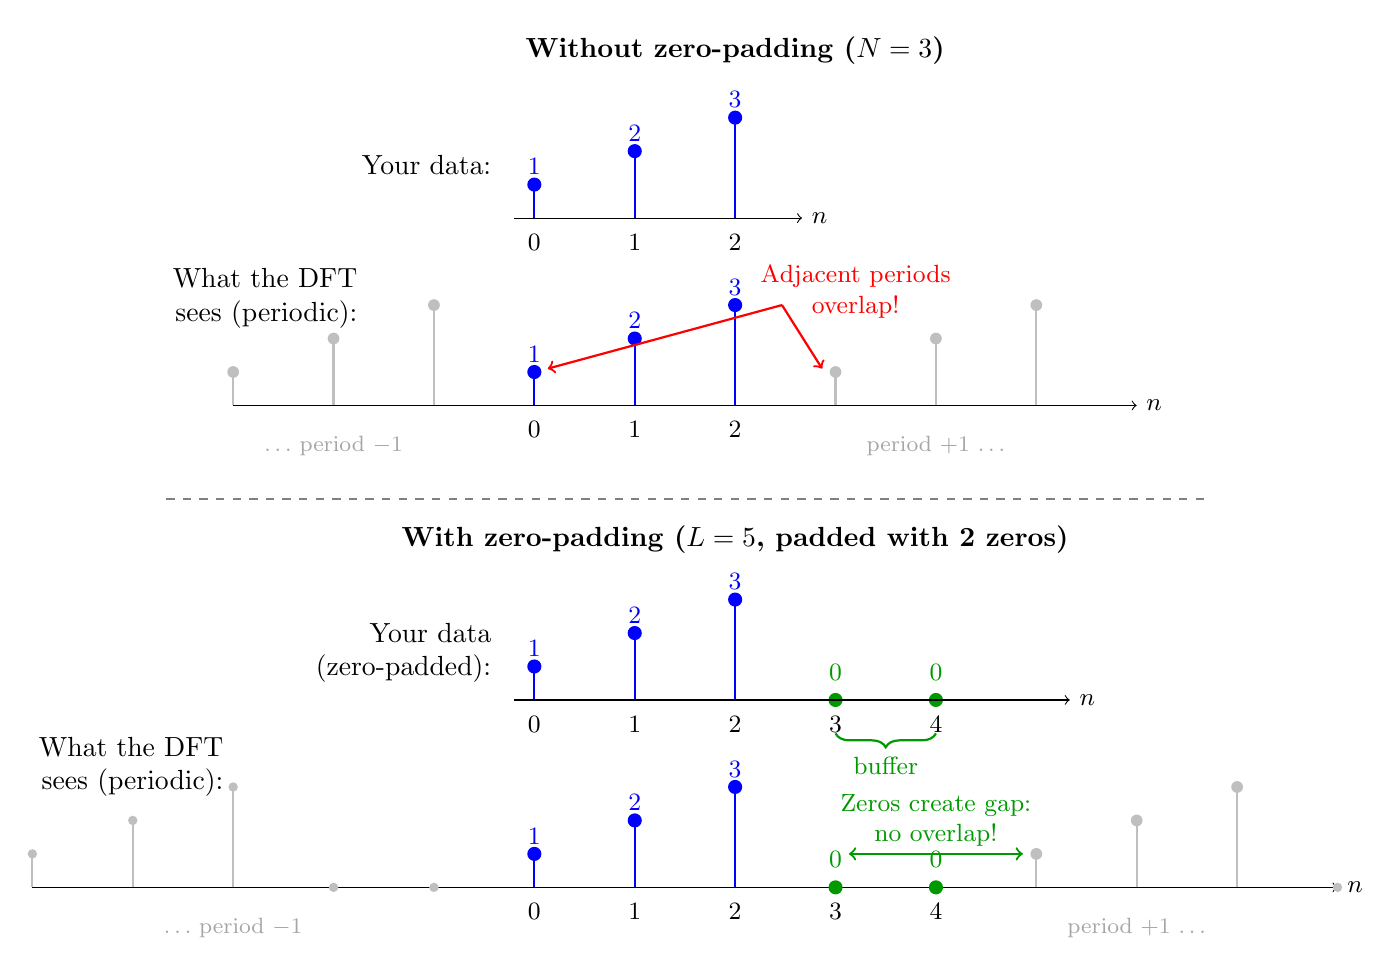
\begin{tikzpicture}[scale=0.85]
    
    % ===== WITHOUT ZERO-PADDING =====
    \node[font=\bfseries] at (3, 5.7) {Without zero-padding ($N=3$)};
    
    % Label for "Your data"
    \node[anchor=east] at (-0.5, 4) {Your data:};
    
    % Draw signal x as stem plot
    \foreach \n/\val in {0/1, 1/2, 2/3} {
        \draw[thick, blue] (\n*1.5, 3.2) -- (\n*1.5, 3.2 + \val*0.5);
        \fill[blue] (\n*1.5, 3.2 + \val*0.5) circle (3pt);
        \node[below, font=\small] at (\n*1.5, 3.1) {$\n$};
        \node[above, font=\small, blue] at (\n*1.5, 3.2 + \val*0.5) {\val};
    }
    \draw[->] (-0.3, 3.2) -- (4, 3.2) node[right, font=\small] {$n$};
    
    % Label for "What DFT sees"
    \node[anchor=east, align=right] at (-2.5, 2) {What the DFT\\sees (periodic):};
    
    % Draw periodic extension
    \draw[->] (-4.5, 0.4) -- (9, 0.4) node[right, font=\small] {$n$};
    
    % Previous period (gray)
    \foreach \n/\val in {0/1, 1/2, 2/3} {
        \pgfmathsetmacro{\xpos}{-4.5 + \n*1.5}
        \draw[thick, gray!50] (\xpos, 0.4) -- (\xpos, 0.4 + \val*0.5);
        \fill[gray!50] (\xpos, 0.4 + \val*0.5) circle (2.5pt);
    }
    \node[gray!70, font=\footnotesize] at (-3, -0.2) {$\ldots$ period $-1$};
    
    % Current period (blue) - indices 0,1,2
    \foreach \n/\val in {0/1, 1/2, 2/3} {
        \draw[thick, blue] (\n*1.5, 0.4) -- (\n*1.5, 0.4 + \val*0.5);
        \fill[blue] (\n*1.5, 0.4 + \val*0.5) circle (3pt);
        \node[below, font=\small] at (\n*1.5, 0.3) {$\n$};
        \node[above, font=\small, blue] at (\n*1.5, 0.4 + \val*0.5) {\val};
    }
    
    % Next period (gray) - shows wrap-around
    \foreach \n/\val in {0/1, 1/2, 2/3} {
        \pgfmathsetmacro{\xpos}{4.5 + \n*1.5}
        \draw[thick, gray!50] (\xpos, 0.4) -- (\xpos, 0.4 + \val*0.5);
        \fill[gray!50] (\xpos, 0.4 + \val*0.5) circle (2.5pt);
    }
    \node[gray!70, font=\footnotesize] at (6, -0.2) {period $+1$ $\ldots$};
    
    % Highlight wrap-around problem
    \draw[red, thick, ->] (3.7, 1.9) -- (4.3, 0.95);
    \draw[red, thick, ->] (3.7, 1.9) -- (0.2, 0.95);
    \node[red, font=\small, align=center] at (4.8, 2.1) {Adjacent periods\\overlap!};
    
    % Vertical separator
    \draw[thick, gray, dashed] (-5.5, -1) -- (10, -1);
    
    % ===== WITH ZERO-PADDING =====
    \node[font=\bfseries] at (3, -1.6) {With zero-padding ($L=5$, padded with 2 zeros)};
    
    % Label for "Your data (padded)"
    \node[anchor=east, align=right] at (-0.5, -3.3) {Your data\\(zero-padded):};
    
    % Draw zero-padded signal
    \foreach \n/\val in {0/1, 1/2, 2/3} {
        \draw[thick, blue] (\n*1.5, -4) -- (\n*1.5, -4 + \val*0.5);
        \fill[blue] (\n*1.5, -4 + \val*0.5) circle (3pt);
        \node[below, font=\small] at (\n*1.5, -4.1) {$\n$};
        \node[above, font=\small, blue] at (\n*1.5, -4 + \val*0.5) {\val};
    }
    % Zeros
    \foreach \n in {3, 4} {
        \draw[thick, green!60!black] (\n*1.5, -4) -- (\n*1.5, -4);
        \fill[green!60!black] (\n*1.5, -4) circle (3pt);
        \node[below, font=\small] at (\n*1.5, -4.1) {$\n$};
        \node[above, font=\small, green!60!black] at (\n*1.5, -3.85) {0};
    }
    \draw[->] (-0.3, -4) -- (8, -4) node[right, font=\small] {$n$};
    
    % Brace for zeros
    \draw[decorate, decoration={brace, amplitude=5pt, mirror}, 
          green!60!black, thick] 
        (4.5, -4.5) -- (6, -4.5) node[midway, below=5pt, 
                                      font=\small, green!60!black] {buffer};
    
    % Label for "What DFT sees"
    \node[anchor=east, align=right] at (-4.5, -5.0) {What the DFT\\sees (periodic):};
    
    % Draw periodic extension with zeros
    \draw[->] (-7.5, -6.8) -- (12, -6.8) node[right, font=\small] {$n$};
    
    % Previous period (gray) with zeros at end
    \foreach \n/\val in {0/1, 1/2, 2/3} {
        \pgfmathsetmacro{\xpos}{-7.5 + \n*1.5}
        \draw[thick, gray!50] (\xpos, -6.8) -- (\xpos, -6.8 + \val*0.5);
        \fill[gray!50] (\xpos, -6.8 + \val*0.5) circle (2pt);
    }
    \foreach \n in {3, 4} {
        \pgfmathsetmacro{\xpos}{-7.5 + \n*1.5}
        \fill[gray!50] (\xpos, -6.8) circle (2pt);
    }
    \node[gray!70, font=\footnotesize] at (-4.5, -7.4) {$\ldots$ period $-1$};
    
    % Current period (blue + green zeros)
    \foreach \n/\val in {0/1, 1/2, 2/3} {
        \draw[thick, blue] (\n*1.5, -6.8) -- (\n*1.5, -6.8 + \val*0.5);
        \fill[blue] (\n*1.5, -6.8 + \val*0.5) circle (3pt);
        \node[below, font=\small] at (\n*1.5, -6.9) {$\n$};
        \node[above, font=\small, blue] at (\n*1.5, -6.8 + \val*0.5) {\val};
    }
    \foreach \n in {3, 4} {
        \fill[green!60!black] (\n*1.5, -6.8) circle (3pt);
        \node[below, font=\small] at (\n*1.5, -6.9) {$\n$};
        \node[above, font=\small, green!60!black] at (\n*1.5, -6.65) {0};
    }
    
    % Next period (gray)
    \foreach \n/\val in {0/1, 1/2, 2/3} {
        \pgfmathsetmacro{\xpos}{7.5 + \n*1.5}
        \draw[thick, gray!50] (\xpos, -6.8) -- (\xpos, -6.8 + \val*0.5);
        \fill[gray!50] (\xpos, -6.8 + \val*0.5) circle (2.5pt);
    }
    \foreach \n in {3} {
        \pgfmathsetmacro{\xpos}{7.5 + \n*1.5}
        \fill[gray!50] (\xpos, -6.8) circle (2pt);
    }
    \node[gray!70, font=\footnotesize] at (9, -7.4) {period $+1$ $\ldots$};
    
    % Show the gap created by zeros
    \draw[green!60!black, thick, <->] (4.7, -6.3) -- (7.3, -6.3);
    \node[green!60!black, font=\small, align=center] at (6, -5.8) 
        {Zeros create gap:\\no overlap!};
    
\end{tikzpicture}
\caption{Zero-padding prevents wrap-around interference. \textbf{Top:} 
         Without padding, the DFT treats the signal as periodic, so 
         adjacent copies overlap during circular convolution. 
         \textbf{Bottom:} With zero-padding, the zeros create a buffer 
         zone between periods, preventing interference.}
\end{figure}

\textbf{Key insight}: When we zero-pad to length $L \geq N+M-1$, the circular convolution 
of the padded signals has no "wrap-around interference" in the first $N+M-1$ samples. 
The zeros act as a buffer that isolates one period from the next in the DFT's implicit 
periodic extension.

\begin{remark}[DFT Periodicity and Zero-Padding]
The DFT formula $X[k] = \sum_{n=0}^{N-1} x[n] e^{-2\pi i kn/N}$ works for \textbf{any} 
sequence $x[n]$ of length $N$. However, the DFT \textbf{interprets} the signal as if it 
were periodic with period $N$. This means mathematically, when we consider indices outside 
$[0, N-1]$, we use $x[n \mod N]$.

With zero-padding, we create a new signal of length $L > N$. The DFT of this padded signal 
treats it as periodic with period $L$. The zeros create a discontinuity at the boundaries, 
but this discontinuity is exactly what creates the "buffer zone" that prevents wrap-around 
interference in circular convolution.

So while the DFT always assumes periodicity, zero-padding ensures that this periodicity 
doesn't cause unwanted interference when computing convolution.
\end{remark}

\subsection{Computational Efficiency: Why This Matters}

Direct linear convolution takes $O(NM)$ operations. Using the FFT with 
zero-padding:

\begin{enumerate}
\item Zero-pad to $L \approx N+M$: $O(L)$
\item Compute $\mathbf{X} = \text{FFT}(\mathbf{x}_{\text{pad}})$: $O(L \log L)$
\item Compute $\mathbf{H} = \text{FFT}(\mathbf{h}_{\text{pad}})$: $O(L \log L)$
\item Multiply: $Y_k = X_k \cdot H_k$: $O(L)$
\item Compute $\mathbf{y} = \text{IFFT}(\mathbf{Y})$: $O(L \log L)$
\end{enumerate}

Total: $O(L \log L)$ instead of $O(NM)$. For large $N, M$, this is a 
dramatic speedup.

\begin{example}[Speedup Comparison]
For $N = M = 10^6$:
\begin{itemize}
\item Direct convolution: $\sim 10^{12}$ operations
\item FFT-based convolution (with $L \approx 2\times10^6$): 
      $\sim 2\times10^6 \times \log_2(2\times10^6) \approx 4\times10^7$ 
      operations
\item Speedup: $\sim 25,000\times$
\end{itemize}
\end{example}

%==========================================================================
\section{Generalization: The Graph Fourier Transform}
%==========================================================================

We've seen that the DFT is the \textit{natural} frequency analysis for the 
circular graph. What about arbitrary graphs? This question leads to 
\textbf{spectral graph theory} \cite{dft-to-gnn:chung1997spectral} and the emerging 
field of signal processing on graphs \cite{dft-to-gnn:shuman2013emerging}.

\subsection{The Key Idea}

The essential insight from the circular case is:

\begin{center}
\fbox{\parbox{0.85\textwidth}{
\textbf{The eigenvectors of the graph Laplacian define a \textit{frequency 
basis} for signals on that graph.}
}}
\end{center}

For the circular graph, these eigenvectors happen to be complex 
exponentials (the DFT basis) because of the special symmetry. For 
general graphs, the eigenvectors are more complicated, but the 
principle is the same.

\subsection{Definition of the Graph Fourier Transform}

\begin{definition}[Graph Fourier Transform]
Let $G$ be a graph with Laplacian $L$ having eigendecomposition:
\begin{equation}
L = U \Lambda U^T
\end{equation}
where $U = [\mathbf{u}_0 | \mathbf{u}_1 | \cdots | \mathbf{u}_{N-1}]$ 
has orthonormal eigenvectors as columns, and 
$\Lambda = \text{diag}(\lambda_0, \ldots, \lambda_{N-1})$ with 
$0 = \lambda_0 \leq \lambda_1 \leq \cdots \leq \lambda_{N-1}$.

The \textbf{Graph Fourier Transform (GFT)} of signal $\mathbf{x}$ is:
\begin{equation}
\hat{\mathbf{x}} = U^T \mathbf{x}
\end{equation}
The \textbf{inverse GFT} is:
\begin{equation}
\mathbf{x} = U \hat{\mathbf{x}}
\end{equation}
\end{definition}

\begin{remark}
The coefficient $\hat{x}_k = \mathbf{u}_k^T \mathbf{x}$ measures how 
much of the $k$-th eigenvector is present in $\mathbf{x}$. Eigenvectors 
with low $\lambda_k$ are ``smooth'' (low variation); those with high 
$\lambda_k$ are ``rough'' (high variation). The GFT decomposes a signal 
into components of increasing ``frequency'' on the graph.
\end{remark}

\subsection{Example: Path Graph}

Consider a path graph with 4 nodes:

\begin{figure}[H]
\centering
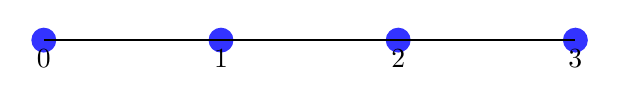
\begin{tikzpicture}[scale=1.5]
    \foreach \i in {0,...,3} {
        \coordinate (n\i) at (\i*1.5, 0);
        \fill[blue!80] (n\i) circle (3pt);
        \node[below] at (n\i) {$\i$};
    }
    \draw[thick] (n0) -- (n1) -- (n2) -- (n3);
\end{tikzpicture}
\caption{Path graph $P_4$.}
\end{figure}

The Laplacian is:
\begin{equation}
L = \begin{pmatrix}
1 & -1 & 0 & 0 \\
-1 & 2 & -1 & 0 \\
0 & -1 & 2 & -1 \\
0 & 0 & -1 & 1
\end{pmatrix}
\end{equation}

The eigenvalues and eigenvectors (exactly) are:

\begin{align*}
\lambda_0 &= 0, \quad \mathbf{u}_0 = \frac{1}{2}(1, 1, 1, 1)^T \\
\lambda_1 &= 2 - \sqrt{2} \approx 0.586, \quad 
           \mathbf{u}_1 \propto (1, \sqrt{2}-1, 1-\sqrt{2}, -1)^T, \\ &\qquad\text{normalized: } \mathbf{u}_1 \approx (0.653, 0.271, -0.271, -0.653)^T \\
\lambda_2 &= 2, \quad \mathbf{u}_2 = \frac{1}{2}(1, -1, -1, 1)^T \\
\lambda_3 &= 2 + \sqrt{2} \approx 3.414, \quad 
           \mathbf{u}_3 \propto (1, -\sqrt{2}-1, \sqrt{2}+1, -1)^T, \\ &\qquad\text{normalized: } \mathbf{u}_3 \approx (0.271, -0.653, 0.653, -0.271)^T
\end{align*}

\begin{figure}[H]
\centering
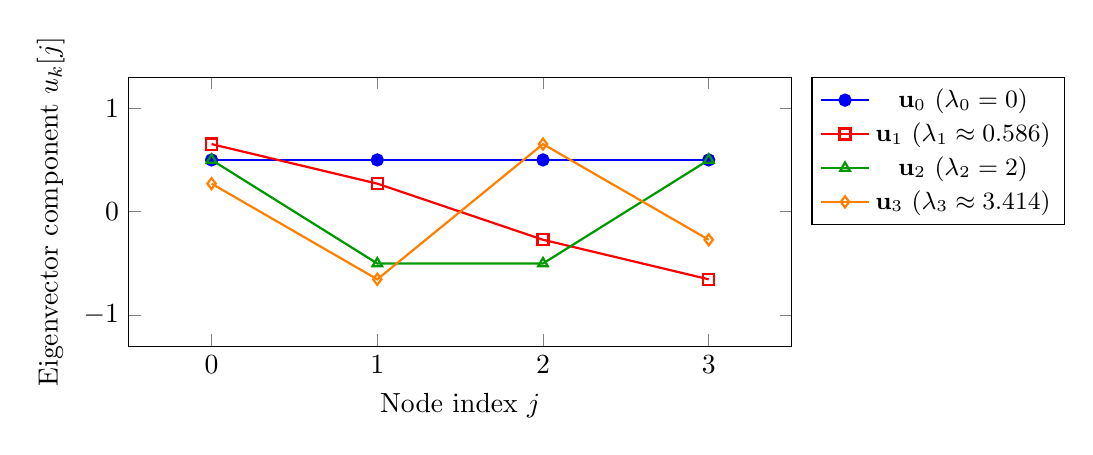
\begin{tikzpicture}
\begin{axis}[
    width=10cm, height=5cm,
    xlabel={Node index $j$},
    ylabel={Eigenvector component $u_k[j]$},
    xmin=-0.5, xmax=3.5,
    ymin=-1.3, ymax=1.3,
    legend pos=outer north east,
    legend style={font=\small},
    xtick={0,1,2,3},
]
% u0
\addplot[thick, blue, mark=*] coordinates {
    (0,0.5) (1,0.5) (2,0.5) (3,0.5)
};
\addlegendentry{$\mathbf{u}_0$ ($\lambda_0=0$)}

% u1
\addplot[thick, red, mark=square] coordinates {
    (0,0.653) (1,0.271) (2,-0.271) (3,-0.653)
};
\addlegendentry{$\mathbf{u}_1$ ($\lambda_1\approx0.586$)}

% u2
\addplot[thick, green!60!black, mark=triangle] coordinates {
    (0,0.5) (1,-0.5) (2,-0.5) (3,0.5)
};
\addlegendentry{$\mathbf{u}_2$ ($\lambda_2=2$)}

% u3
\addplot[thick, orange, mark=diamond] coordinates {
    (0,0.271) (1,-0.653) (2,0.653) (3,-0.271)
};
\addlegendentry{$\mathbf{u}_3$ ($\lambda_3\approx3.414$)}
\end{axis}
\end{tikzpicture}
\caption{Eigenvectors of the path graph $P_4$. These look like discretized
         cosines, similar to DFT basis vectors but adapted to the path's
         boundary conditions.}
\end{figure}

These eigenvectors look like discretized cosines---similar to the DFT, 
but adapted to the boundary conditions of the path. This is not a 
coincidence: the path graph eigenvectors are exactly the Discrete 
Cosine Transform (DCT) basis (see Appendix~\ref{dft-to-gnn:app:dct-path}). Notice that:
\begin{itemize}
    \item $\mathbf{u}_0$ is constant (like $k=0$ in DFT)
    \item $\mathbf{u}_1$ has one "bump" (like $k=1$ in DFT)
    \item $\mathbf{u}_2$ has two "bumps" (like $k=2$ in DFT)
    \item $\mathbf{u}_3$ has three "bumps" (like $k=3$ in DFT) 
\end{itemize}

%==========================================================================
\section{Spectral Graph Convolution}
%==========================================================================

\subsection{The Problem: What is Convolution on a Graph?}

On regular structures (like the circle or grid), convolution slides a 
filter across the signal. But on an irregular graph, there's no 
consistent notion of ``sliding''---the neighborhood structure varies 
from node to node.

However, we can define convolution \emph{spectrally}:

\begin{center}
\fbox{\parbox{0.85\textwidth}{
\textbf{Spectral Convolution}: Since convolution becomes multiplication 
in the frequency domain, we \emph{define} graph convolution as 
multiplication in the Graph Fourier domain.
}}
\end{center}

\subsection{Definition of Spectral Graph Convolution}

\begin{definition}[Spectral Graph Convolution]
The spectral convolution of signal $\mathbf{x}$ with filter $g$ on 
graph $G$ is:
\begin{equation}
\mathbf{x} *_G g = U \, g(\Lambda) \, U^T \mathbf{x}
\end{equation}
where $g(\Lambda) = \text{diag}(g(\lambda_0), g(\lambda_1), \ldots, 
g(\lambda_{N-1}))$ is the filter applied to each eigenvalue.
\end{definition}

In other words:
\begin{enumerate}
\item Transform to the graph spectral domain: 
      $\hat{\mathbf{x}} = U^T \mathbf{x}$
\item Multiply by the filter's frequency response: 
      $\hat{\mathbf{y}}_k = g(\lambda_k) \cdot \hat{\mathbf{x}}_k$
\item Transform back: $\mathbf{y} = U \hat{\mathbf{y}}$
\end{enumerate}

\subsection{Example Filters: Why These Work as Low/High-Pass Filters}

The choice of filter function $g(\lambda)$ determines what kind of 
operation we perform on the graph signal. Here's a detailed explanation 
of why certain functions act as low-pass or high-pass filters:

\begin{itemize}
\item \textbf{Low-pass filter: $g(\lambda) = e^{-\alpha \lambda}$} \\
This is the graph equivalent of a Gaussian filter. Recall that eigenvalues 
$\lambda_k$ measure how "rough" a signal component is:
\begin{itemize}
    \item Small $\lambda$ $\rightarrow$ smooth eigenvectors (low frequency)
    \item Large $\lambda$ $\rightarrow$ rough eigenvectors (high frequency)
\end{itemize}
For $g(\lambda) = e^{-\alpha \lambda}$:
\begin{itemize}
    \item When $\lambda \approx 0$: $g(0) = e^0 = 1$ (fully preserved)
    \item When $\lambda$ is large: $g(\lambda) \approx 0$ (heavily attenuated)
\end{itemize}
Thus, smooth (low-frequency) components are preserved, while rough 
(high-frequency) components are suppressed---exactly what a low-pass 
filter should do.

\item \textbf{Alternative low-pass: $g(\lambda) = \frac{1}{1 + \alpha\lambda}$} \\
This has similar properties but with a rational form. As $\lambda \to 0$, 
$g(\lambda) \to 1$; as $\lambda \to \infty$, $g(\lambda) \to 0$. This is 
sometimes called the "graph heat kernel" when $\alpha = t$ (time parameter).

\item \textbf{High-pass filter: $g(\lambda) = 1 - e^{-\alpha \lambda}$} \\
This is the complement of the low-pass filter:
\begin{itemize}
    \item When $\lambda \approx 0$: $g(0) = 1 - 1 = 0$ (suppressed)
    \item When $\lambda$ is large: $g(\lambda) \approx 1$ (preserved)
\end{itemize}
Thus, smooth components are suppressed while rough components are 
preserved---exactly a high-pass filter.

\item \textbf{Heat diffusion: $g(\lambda) = e^{-t\lambda}$} \\
This has a physical interpretation: imagine heat diffusing on the graph 
over time $t$. Starting from an initial temperature distribution $\mathbf{x}$, 
after time $t$, the temperature becomes $\mathbf{y} = U e^{-t\Lambda} U^T \mathbf{x}$. 
Large $t$ gives more smoothing (like low-pass filtering).

\item \textbf{Polynomial filter: $g(\lambda) = \sum_{k=0}^{K-1} \theta_k \lambda^k$} \\
This is particularly important because it can be computed \emph{without} 
full eigendecomposition. Notice that:
\[
U g(\Lambda) U^T = U\left(\sum_{k=0}^{K-1} \theta_k \Lambda^k\right) U^T 
= \sum_{k=0}^{K-1} \theta_k U\Lambda^k U^T 
= \sum_{k=0}^{K-1} \theta_k L^k
\]
where we used $L = U\Lambda U^T$ and thus $L^k = U\Lambda^k U^T$.

\textbf{Why computing $L^k$ is efficient}: 
\begin{itemize}
    \item We don't need to compute eigenvectors $U$ at all
    \item $L^k\mathbf{x}$ can be computed recursively: $L(L^{k-1}\mathbf{x})$
    \item Each multiplication by $L$ is sparse (only involves neighbors)
    \item $L^k\mathbf{x}$ aggregates information from $k$-hop neighborhoods
\end{itemize}
\end{itemize}

\begin{figure}[H]
\centering
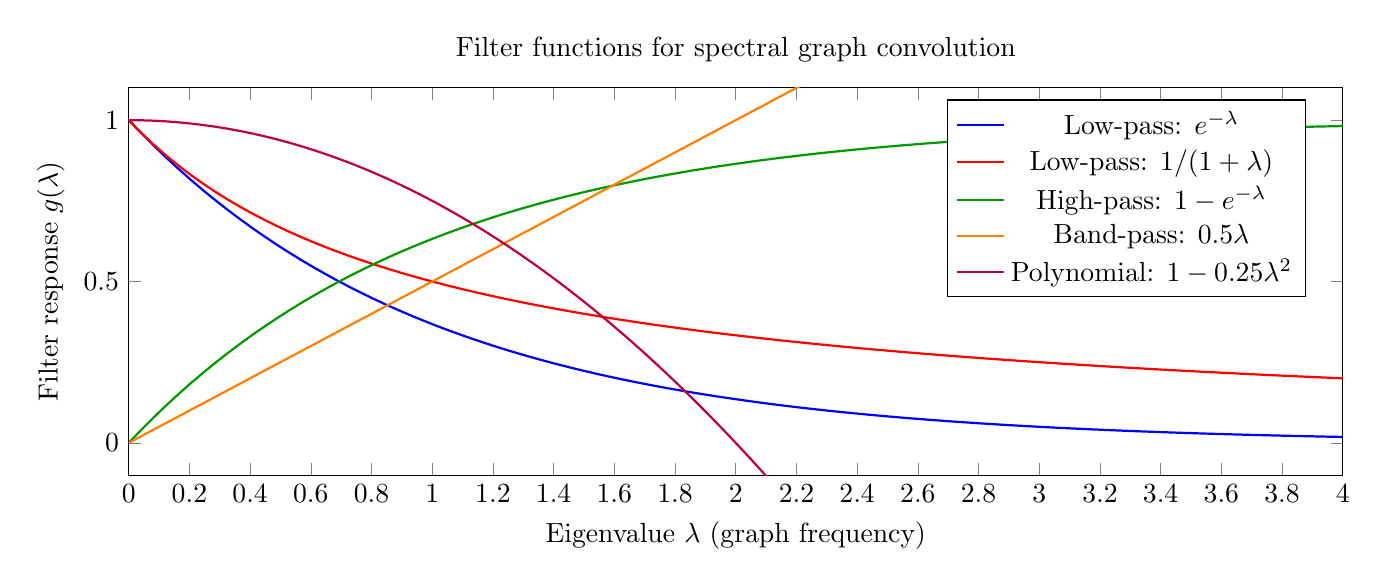
\begin{tikzpicture}
\begin{axis}[
    width=17cm, height=6.5cm,
    xlabel={Eigenvalue $\lambda$ (graph frequency)},
    ylabel={Filter response $g(\lambda)$},
    xmin=0, xmax=4,
    ymin=-0.1, ymax=1.1,
    legend pos=north east,
    title={Filter functions for spectral graph convolution},
]
\addplot[thick, blue, domain=0:4, samples=100] {exp(-x)};
\addlegendentry{Low-pass: $e^{-\lambda}$}
\addplot[thick, red, domain=0:4, samples=100] {1/(1+x)};
\addlegendentry{Low-pass: $1/(1+\lambda)$}
\addplot[thick, green!60!black, domain=0:4, samples=100] {1 - exp(-x)};
\addlegendentry{High-pass: $1 - e^{-\lambda}$}
\addplot[thick, orange, domain=0:4, samples=100] {0.5*x};
\addlegendentry{Band-pass: $0.5\lambda$}
\addplot[thick, purple, domain=0:4, samples=100] {1 - 0.25*x^2};
\addlegendentry{Polynomial: $1 - 0.25\lambda^2$}
\end{axis}
\end{tikzpicture}
\caption{Filter functions for spectral graph convolution. Low-pass filters 
         (blue, red) preserve small $\lambda$ (smooth components) and attenuate 
         large $\lambda$ (rough components). High-pass filters (green) do the 
         opposite. Polynomial filters (purple) can approximate various shapes.}
\end{figure}

\subsection{Why Polynomial Filters are Crucial: Computational Efficiency}

The full spectral convolution $\mathbf{y} = U g(\Lambda) U^T \mathbf{x}$ requires:
\begin{enumerate}
\item Computing eigendecomposition $L = U\Lambda U^T$: $O(N^3)$ operations
\item Applying $U^T$ and $U$: $O(N^2)$ each
\end{enumerate}
For large graphs (millions of nodes), this is impossible.

However, if $g(\lambda)$ is a \textbf{polynomial} of degree $K-1$:
\[
g(\lambda) = \sum_{k=0}^{K-1} \theta_k \lambda^k
\]
then:
\[
U g(\Lambda) U^T = \sum_{k=0}^{K-1} \theta_k U\Lambda^k U^T = \sum_{k=0}^{K-1} \theta_k L^k
\]
No eigendecomposition needed! We only need to compute $L^k \mathbf{x}$ for 
$k = 0, 1, \ldots, K-1$.

\textbf{What does $L^k \mathbf{x}$ compute?}
Recall that $(L\mathbf{x})_i = \sum_{j \sim i} A_{ij}(x_i - x_j)$ measures 
local variation. Then:
\begin{itemize}
\item $L^0\mathbf{x} = \mathbf{x}$ (the signal itself)
\item $L^1\mathbf{x}$ aggregates information from immediate neighbors
\item $L^2\mathbf{x} = L(L\mathbf{x})$ aggregates from 2-hop neighbors
\item $L^k\mathbf{x}$ aggregates information from $k$-hop neighbors
\end{itemize}

So polynomial filters of degree $K-1$ combine information from up to 
$(K-1)$-hop neighborhoods, with weights $\theta_k$ learned from data.

\subsection{Verification: Recovering Classical Convolution}

On the circular graph, $U = F^*/\sqrt{N}$ (the normalized DFT matrix) 
and $\Lambda$ contains the eigenvalues $\lambda_k = 4\sin^2(\pi k/N)$. 
If we choose a filter that depends on $k$ rather than $\lambda_k$, we 
recover exactly the classical convolution theorem.

\begin{example}[Circular Convolution as Special Case]
For the circular graph, let $g(\lambda_k) = H_k$ where $H_k$ is the 
DFT of some filter $\mathbf{h}$. Then:
\begin{align*}
\mathbf{x} *_G g &= U \, \text{diag}(H_0, \ldots, H_{N-1}) \, U^T \mathbf{x} \\
&= \frac{1}{\sqrt{N}} F^* \, \text{diag}(\mathbf{H}) \, 
   \frac{1}{\sqrt{N}} F \mathbf{x} \\
&= F^{-1} \, \text{diag}(\mathbf{H}) \, F \mathbf{x} \\
&= C_h \mathbf{x} = \mathbf{x} \circledast \mathbf{h}
\end{align*}
which is exactly circular convolution.
\end{example}

\subsection{Example: Applying a Low-Pass Filter on a Path Graph}

Let's apply a low-pass filter $g(\lambda) = e^{-\lambda}$ to a signal 
on the path graph $P_4$.

\begin{example}[Spectral Convolution on $P_4$]
Consider the path graph $P_4$ with signal $\mathbf{x} = [1, 0, 0, 0]^T$ 
(a unit impulse at node 0). We want to smooth this signal using a 
low-pass filter $g(\lambda) = e^{-\lambda}$.

From our earlier calculation (the DCT-II basis of \cref{dft-to-gnn:thm:path-dct} with $N = 4$), the
orthonormal eigenvectors and the eigenvalues are:
\begin{align*}
\lambda_0 &= 0, \quad \mathbf{u}_0 = \tfrac{1}{2}(1, 1, 1, 1)^T \\
\lambda_1 &= 2 - \sqrt{2} \approx 0.586, \quad \mathbf{u}_1 \approx (0.653, 0.271, -0.271, -0.653)^T \\
\lambda_2 &= 2, \quad \mathbf{u}_2 = \tfrac{1}{2}(1, -1, -1, 1)^T \\
\lambda_3 &= 2 + \sqrt{2} \approx 3.414, \quad \mathbf{u}_3 \approx (0.271, -0.653, 0.653, -0.271)^T
\end{align*}
(The graph Fourier transform requires an \emph{orthonormal} basis: the vectors must be normalized.)

\textbf{Step 1: Graph Fourier Transform}
\[
\hat{\mathbf{x}} = U^T \mathbf{x} =
\begin{pmatrix}
\mathbf{u}_0^T \mathbf{x} \\
\mathbf{u}_1^T \mathbf{x} \\
\mathbf{u}_2^T \mathbf{x} \\
\mathbf{u}_3^T \mathbf{x}
\end{pmatrix}
\approx
\begin{pmatrix}
0.5 \\
0.653 \\
0.5 \\
0.271
\end{pmatrix}
\]
Since $\mathbf{x}$ is the impulse at node 0, $\hat{x}_k = u_k[0]$: the impulse contains \emph{all}
frequencies, but not with equal weights (unlike the classical DFT, where an impulse has a flat spectrum,
the graph eigenvectors do not all have the same magnitude at node 0).

\textbf{Step 2: Apply filter in frequency domain}
\[
g(\Lambda) = \text{diag}(e^0, e^{-0.586}, e^{-2}, e^{-3.414})
\approx \text{diag}(1, 0.557, 0.135, 0.033)
\]
\[
\hat{\mathbf{y}} = g(\Lambda) \hat{\mathbf{x}} \approx
\begin{pmatrix}
1 \times 0.5 \\
0.557 \times 0.653 \\
0.135 \times 0.5 \\
0.033 \times 0.271
\end{pmatrix}
\approx
\begin{pmatrix}
0.5 \\
0.364 \\
0.068 \\
0.009
\end{pmatrix}
\]

\textbf{Step 3: Inverse Graph Fourier Transform}
\[
\mathbf{y} = U \hat{\mathbf{y}} = 0.5\mathbf{u}_0 + 0.364\mathbf{u}_1 +
0.068\mathbf{u}_2 + 0.009\mathbf{u}_3
\]
Approximately:
\[
\mathbf{y} \approx
\begin{pmatrix}
    0.25+0.238+0.034+0.002\\
    0.25+0.098-0.034-0.006\\
    0.25-0.098-0.034+0.006\\
    0.25-0.238+0.034-0.002
\end{pmatrix}
\]
\[
\mathbf{y} \approx [0.524, 0.309, 0.124, 0.044]^T
\]
This is $e^{-L}\mathbf{x}$, the heat kernel applied to the impulse (checked numerically). Note that the
entries still sum to $1$: since $L\mathbf{1} = \mathbf{0}$, heat diffusion conserves the total ``mass'' of the
signal.

The impulse has been smoothed across the graph! The low-pass filter 
attenuated high-frequency components, spreading the energy from node 0 
to its neighbors.
\end{example}

%==========================================================================
\section{Application: Graph Convolutional Networks}
%==========================================================================

\subsection{The Machine Learning Context}

In many applications, data naturally lives on graphs:
\begin{itemize}
\item Social networks: users and friendships
\item Molecules: atoms and bonds
\item Citation networks: papers and references
\item Knowledge graphs: entities and relations
\end{itemize}

We want neural networks that can process such data while respecting 
the graph structure---analogous to how CNNs process images while 
respecting the grid structure.

\subsection{Spectral Graph Neural Networks}

The spectral approach to graph convolution gives us:

\begin{definition}[Spectral Graph Convolutional Layer]
Given input signal $\mathbf{x} \in \R^N$ and learnable filter 
$g_\theta$:
\begin{equation}
\mathbf{y} = \sigma\left( U \, g_\theta(\Lambda) \, U^T \mathbf{x} 
             \right)
\end{equation}
where $\sigma$ is a nonlinearity (e.g., ReLU).
\end{definition}

\textbf{Problem}: Computing the full eigendecomposition 
$L = U\Lambda U^T$ costs $O(N^3)$. For large graphs, this is 
prohibitive.

\subsection{ChebNet: Using Chebyshev Polynomials}

We've seen that polynomial filters $g(\lambda) = \sum_{k=0}^{K-1} 
\theta_k \lambda^k$ avoid eigendecomposition. ChebNet \cite{dft-to-gnn:defferrard2016convolutional} improves on this 
by using \textbf{Chebyshev polynomials} instead of the standard monomial 
basis.

\subsubsection{Why Change the Polynomial Basis?}

Any polynomial of degree $K-1$ can be written either as:
\[
\sum_{k=0}^{K-1} a_k \lambda^k \quad \text{(monomial basis)}
\qquad \text{or} \qquad
\sum_{k=0}^{K-1} b_k T_k(\lambda) \quad \text{(Chebyshev basis)}
\]

These are just two different ways to parameterize the \emph{same} set 
of polynomials. So why prefer Chebyshev?

\begin{enumerate}
\item \textbf{Numerical stability}: The monomials $\lambda^k$ can grow 
      very large or very small, causing numerical issues. Chebyshev 
      polynomials satisfy $|T_k(x)| \leq 1$ for $x \in [-1, 1]$.

\item \textbf{Efficient recurrence}: Chebyshev polynomials satisfy
      \[
      T_0(x) = 1, \quad T_1(x) = x, \quad 
      T_{k+1}(x) = 2x \cdot T_k(x) - T_{k-1}(x)
      \]
      This allows computing $T_k(\tilde{L})\mathbf{x}$ recursively without 
      storing or computing high powers of $L$.

\item \textbf{Orthogonality}: Chebyshev polynomials are orthogonal 
      with respect to a certain weight, which can help optimization.
\end{enumerate}

\subsubsection{The Rescaling Step}

Chebyshev polynomials are well-behaved on $[-1, 1]$, but the eigenvalues 
of $L$ lie in $[0, \lambda_{\max}]$. We therefore rescale:

\begin{equation}
\tilde{\lambda} = \frac{2\lambda}{\lambda_{\max}} - 1 
\quad \in [-1, 1]
\end{equation}

Equivalently, we define the rescaled Laplacian:
\begin{equation}
\tilde{L} = \frac{2L}{\lambda_{\max}} - I
\end{equation}

The ChebNet filter is then:
\begin{equation}
\mathbf{y} = \sum_{k=0}^{K-1} \theta_k \, T_k(\tilde{L}) \, \mathbf{x}
\end{equation}

\subsubsection{Efficient Computation via Recurrence}

Using the Chebyshev recurrence, we compute:
\begin{align}
\bar{\mathbf{x}}_0 &= \mathbf{x} \\
\bar{\mathbf{x}}_1 &= \tilde{L} \mathbf{x} \\
\bar{\mathbf{x}}_k &= 2\tilde{L} \bar{\mathbf{x}}_{k-1} - \bar{\mathbf{x}}_{k-2}
\end{align}

Then:
\[
\mathbf{y} = \sum_{k=0}^{K-1} \theta_k \bar{\mathbf{x}}_k
\]

This requires only $K$ sparse matrix-vector multiplications with $L$, 
giving complexity $O(K \cdot |E|)$ instead of $O(N^3)$.

\begin{example}[ChebNet Computation on a Triangle Graph]
Consider a triangle graph (3 nodes, each connected to the other two) 
with signal $\mathbf{x} = [1, 0, 0]^T$ (a unit impulse at node 0).

\begin{center}
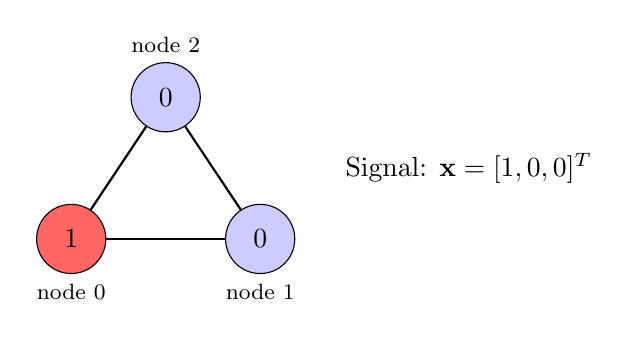
\begin{tikzpicture}[scale=1.2]
    % Nodes
    \node[circle, draw, fill=red!60, minimum size=25pt] (n0) at (0, 0) {$1$};
    \node[circle, draw, fill=blue!20, minimum size=25pt] (n1) at (2, 0) {$0$};
    \node[circle, draw, fill=blue!20, minimum size=25pt] (n2) at (1, 1.5) {$0$};
    
    % Edges
    \draw[thick] (n0) -- (n1);
    \draw[thick] (n1) -- (n2);
    \draw[thick] (n2) -- (n0);
    
    % Labels
    \node[below] at (n0.south) {\footnotesize node 0};
    \node[below] at (n1.south) {\footnotesize node 1};
    \node[above] at (n2.north) {\footnotesize node 2};
    
    % Signal annotation
    \node[right] at (2.8, 0.75) {Signal: $\mathbf{x} = [1, 0, 0]^T$};
\end{tikzpicture}
\end{center}

The Laplacian is:
\[
L = \begin{pmatrix} 2 & -1 & -1 \\ -1 & 2 & -1 \\ -1 & -1 & 2 \end{pmatrix}
\]
with $\lambda_{\max} = 3$. The rescaled Laplacian is:
\[
\tilde{L} = \frac{2}{3}L - I = 
\begin{pmatrix} 1/3 & -2/3 & -2/3 \\ -2/3 & 1/3 & -2/3 \\ -2/3 & -2/3 & 1/3 \end{pmatrix}
\]

For $K=3$ (degree-2 polynomial), we compute:

\textbf{Step 1}: $\bar{\mathbf{x}}_0 = T_0(\tilde{L})\mathbf{x} = \mathbf{x} = [1, 0, 0]^T$

\textbf{Step 2}: $\bar{\mathbf{x}}_1 = T_1(\tilde{L})\mathbf{x} = \tilde{L}\mathbf{x} = [1/3, -2/3, -2/3]^T$

\textbf{Step 3}: $\bar{\mathbf{x}}_2 = 2\tilde{L}\bar{\mathbf{x}}_1 - \bar{\mathbf{x}}_0$
\[
= 2 \begin{pmatrix} 1/3 \\ -2/3 \\ -2/3 \end{pmatrix} \cdot \frac{1}{3}
+ 2 \begin{pmatrix} -2/3 \\ 1/3 \\ -2/3 \end{pmatrix} \cdot (-\frac{2}{3})
+ 2 \begin{pmatrix} -2/3 \\ -2/3 \\ 1/3 \end{pmatrix} \cdot (-\frac{2}{3})
- \begin{pmatrix} 1 \\ 0 \\ 0 \end{pmatrix}
= \begin{pmatrix} -1/9 \\ -4/9 \\ -4/9 \end{pmatrix}
\]

\textbf{Step 4}: Output with learned weights $\theta_0, \theta_1, \theta_2$:
\[
\mathbf{y} = \theta_0 \begin{pmatrix} 1 \\ 0 \\ 0 \end{pmatrix}
+ \theta_1 \begin{pmatrix} 1/3 \\ -2/3 \\ -2/3 \end{pmatrix}
+ \theta_2 \begin{pmatrix} -1/9 \\ -4/9 \\ -4/9 \end{pmatrix}
\]

The key point: we computed this using only 2 sparse matrix-vector 
multiplications with $\tilde{L}$, never touching eigenvectors!
\end{example}

\subsection{GCN: The Simplified First-Order Case}

The Graph Convolutional Network (GCN) \cite{dft-to-gnn:kipf2017semi} 
simplifies ChebNet by using $K=1$ (only first-order neighbors) and 
making additional approximations.

Starting from a first-order Chebyshev filter ($K=2$ terms, but we'll 
reduce parameters):

\[
\mathbf{y} = \theta_0 \mathbf{x} + \theta_1 \tilde{L} \mathbf{x}
\]
where $\tilde{L} = \frac{2}{\lambda_{\max}}L - I$ is the rescaled Laplacian.

GCN makes two simplifying assumptions:
\begin{enumerate}
\item $\lambda_{\max} \approx 2$ (true for many normalized graphs)
\item $\theta = \theta_0 = -\theta_1$ (tie the parameters)
\end{enumerate}

With these assumptions and $\lambda_{\max} = 2$, we have 
$\tilde{L} = L - I$, so:
\[
\mathbf{y} = \theta \mathbf{x} - \theta(L - I)\mathbf{x} 
           = \theta(2I - L)\mathbf{x}
           = \theta(I + D^{-1/2} A D^{-1/2})\mathbf{x}
\]
where $A$ is the adjacency matrix and $D$ is the degree matrix. This 
uses the normalized Laplacian $L = I - D^{-1/2} A D^{-1/2}$.

\subsubsection{From Filter to Neural Network Layer}

The expression $\theta(I + D^{-1/2} A D^{-1/2})\mathbf{x}$ is a spectral 
filter with a single learnable parameter $\theta$. To turn this into a 
useful neural network layer, we make three modifications:

\textbf{Step 1: Renormalization trick.} The term $I + D^{-1/2} A D^{-1/2}$ 
combines the normalized adjacency with the identity. However, this can 
lead to numerical instabilities (eigenvalues in $[0, 2]$ instead of 
$[0, 1]$). Kipf \& Welling \cite{dft-to-gnn:kipf2017semi} proposed a "renormalization trick": instead 
of adding $I$ after normalizing, add self-loops \emph{before} normalizing. 
Define:
\begin{itemize}
    \item $\hat{A} = A + I$ (adjacency matrix with self-loops added)
    \item $\hat{D}$ = degree matrix of $\hat{A}$ (i.e., 
          $\hat{D}_{ii} = \sum_j \hat{A}_{ij} = D_{ii} + 1$)
\end{itemize}
Then use $\hat{D}^{-1/2} \hat{A} \hat{D}^{-1/2}$ instead of 
$I + D^{-1/2} A D^{-1/2}$. This keeps eigenvalues in $[-1, 1]$ and 
improves training stability.

\textbf{Step 2: Replace scalar $\theta$ with weight matrix $W$.} 
Instead of a single scalar parameter, we use a learnable weight matrix 
$W \in \mathbb{R}^{d \times d'}$ that transforms $d$-dimensional input 
features to $d'$-dimensional output features. This allows the layer to 
learn rich feature transformations.

\textbf{Step 3: Add nonlinearity.} To enable the network to learn 
nonlinear functions, we apply an activation function $\sigma$ (typically 
ReLU) after the linear transformation.

\textbf{The final GCN layer} combines these three modifications:

\begin{equation}
H^{(l+1)} = \sigma\left( \hat{D}^{-1/2} \hat{A} \hat{D}^{-1/2} 
             H^{(l)} W^{(l)} \right)
\end{equation}

where:
\begin{itemize}
    \item $H^{(l)} \in \mathbb{R}^{N \times d}$ is the matrix of node 
          features at layer $l$ ($N$ nodes, $d$ features each)
    \item $W^{(l)} \in \mathbb{R}^{d \times d'}$ is the learnable weight 
          matrix for layer $l$
    \item $\sigma$ is a nonlinear activation (e.g., ReLU)
    \item $H^{(l+1)} \in \mathbb{R}^{N \times d'}$ is the output
\end{itemize}

\begin{remark}[From Scalars to Matrices]
In the original spectral filter, each node had a scalar signal value 
$x_i$, and $\theta$ was a scalar parameter. In the GCN layer:
\begin{itemize}
    \item Each node has a \emph{feature vector} $\mathbf{h}_i \in \mathbb{R}^d$, 
          so we stack them into a matrix $H \in \mathbb{R}^{N \times d}$
    \item The scalar $\theta$ becomes a \emph{weight matrix} 
          $W \in \mathbb{R}^{d \times d'}$ that transforms features
\end{itemize}
\end{remark}

\begin{example}[GCN Layer on a Small Graph]
Consider a 4-node graph where each node has 2 features:

\begin{center}
\begin{tikzpicture}[scale=1.0]
    \node[circle, draw, fill=red!30, minimum size=25pt] (n0) at (0, 1) {0};
    \node[circle, draw, fill=green!30, minimum size=25pt] (n1) at (2, 1) {1};
    \node[circle, draw, fill=blue!30, minimum size=25pt] (n2) at (2, -0.5) {2};
    \node[circle, draw, fill=orange!30, minimum size=25pt] (n3) at (0, -0.5) {3};
    \draw[thick] (n0) -- (n1);
    \draw[thick] (n1) -- (n2);
    \draw[thick] (n2) -- (n3);
    \draw[thick] (n3) -- (n0);
    \draw[thick] (n0) -- (n2);
    
    % Feature annotations
    \node[right, font=\small] at (2.8, 0.8) {
        $H^{(0)} = \begin{pmatrix} 
        1 & 0 \\ 0 & 1 \\ 1 & 1 \\ 0 & 0 
        \end{pmatrix}$};
    \node[right, font=\small] at (2.8, -0.2) {\footnotesize (4 nodes, 2 features)};
\end{tikzpicture}
\end{center}

\textbf{Step 1: Compute $\hat{A}$ and $\hat{D}$.}

Adjacency matrix and with self-loops:
\[
A = \begin{pmatrix} 
0 & 1 & 1 & 1 \\ 
1 & 0 & 1 & 0 \\ 
1 & 1 & 0 & 1 \\ 
1 & 0 & 1 & 0 
\end{pmatrix}, \quad
\hat{A} = A + I = \begin{pmatrix} 
1 & 1 & 1 & 1 \\ 
1 & 1 & 1 & 0 \\ 
1 & 1 & 1 & 1 \\ 
1 & 0 & 1 & 1 
\end{pmatrix}
\]

Degrees: $\hat{D} = \text{diag}(4, 3, 4, 3)$.

\textbf{Step 2: Compute the normalized adjacency.}
\[
\hat{D}^{-1/2} \hat{A} \hat{D}^{-1/2} =
{
\renewcommand{\arraystretch}{1.5} % Increases row height
\setlength{\arraycolsep}{4pt}    % Adjusts column width
\begin{pmatrix} 
\frac{1}{4} & \frac{1}{2\sqrt{3}} & \frac{1}{4} & \frac{1}{2\sqrt{3}} \\ 
\frac{1}{2\sqrt{3}} & \frac{1}{3} & \frac{1}{2\sqrt{3}} & 0 \\ 
\frac{1}{4} & \frac{1}{2\sqrt{3}} & \frac{1}{4} & \frac{1}{2\sqrt{3}} \\ 
\frac{1}{2\sqrt{3}} & 0 & \frac{1}{2\sqrt{3}} & \frac{1}{3} 
\end{pmatrix}
=
\begin{pmatrix} 
0.25 & 0.29 & 0.25 & 0.29 \\ 
0.29 & 0.33 & 0.29 & 0 \\ 
0.25 & 0.29 & 0.25 & 0.29 \\ 
0.29 & 0 & 0.29 & 0.33 
\end{pmatrix}
}
\]
(entries rounded to 2 decimal places)

\textbf{Step 3: Apply GCN layer.} With weight matrix 
$W = \begin{pmatrix} 1 & 0 \\ 0 & 1 \end{pmatrix}$ (identity, for simplicity):

\[
H^{(1)} = \sigma\left( \hat{D}^{-1/2} \hat{A} \hat{D}^{-1/2} H^{(0)} W \right)
\]

First, aggregate features (before nonlinearity):
\[
\hat{D}^{-1/2} \hat{A} \hat{D}^{-1/2} H^{(0)} = 
\begin{pmatrix} 
0.25 + 0.25 & 0.29 + 0.25 \\
0.29 + 0.29 & 0.33 + 0.29 \\
0.25 + 0.29 + 0.25 & 0.29 + 0.25 + 0.29 \\
0.29 + 0.29 & 0.29
\end{pmatrix}
= \begin{pmatrix} 
0.50 & 0.54 \\
0.58 & 0.62 \\
0.79 & 0.83 \\
0.58 & 0.29
\end{pmatrix}
\]

Each row is now a weighted average of that node's features and its 
neighbors' features. Applying ReLU (all values positive, so unchanged):
\[
H^{(1)} = \begin{pmatrix} 
0.50 & 0.54 \\
0.58 & 0.62 \\
0.79 & 0.83 \\
0.58 & 0.29
\end{pmatrix}
\]

Node 2 (connected to all others) aggregates the most information. 
Node 3 (only connected to nodes 0 and 2) has lower values in the 
second feature.
\end{example}

\subsubsection{Interpretation of GCN}

The GCN layer can be interpreted as:
\begin{enumerate}
\item \textbf{Feature transformation}: Multiply by $W$ to learn 
      new feature representations
\item \textbf{Neighborhood aggregation}: Multiply by 
      $\hat{D}^{-1/2} \hat{A} \hat{D}^{-1/2}$ to average each node's 
      features with its neighbors' features
\item \textbf{Nonlinearity}: Apply $\sigma$ (e.g., ReLU) to enable 
      nonlinear decision boundaries
\end{enumerate}

This simple formulation has proven remarkably effective in practice and 
forms the basis for many modern GNN architectures.

\subsection{Summary: The Spectral Foundation of GNNs}

\begin{center}
\begin{tikzpicture}[node distance=1.8cm, auto,
    block/.style={rectangle, draw, fill=blue!10, , align=center,
                  text width=5em, text centered, minimum height=2.5em,
                  rounded corners=3pt},
    arrow/.style={->, >=stealth, thick, align=center}]
    
    \node[block] (dft) {DFT on Circle};
    \node[block, right=of dft] (gft) {Graph Fourier\\Transform};
    \node[block, right=of gft] (spec) {Spectral Graph\\Convolution};
    \node[block, right=of spec] (cheb) {ChebNet\\($K$-polynomial)};
    \node[block, right=of cheb] (gcn) {GCN\\($K=1$ approx)};
    
    \draw[arrow] (dft) -- node[above] {Generalize} (gft);
    \draw[arrow] (gft) -- node[above] {Define} (spec);
    \draw[arrow] (spec) -- node[above] {Polynomial\\approx} (cheb);
    \draw[arrow] (cheb) -- node[above] {Simplify} (gcn);
    
    \node[below=0.3cm of dft] {\footnotesize Basis: $e^{2\pi i kn/N}$};
    \node[below=0.3cm of gft] {\footnotesize Basis: eigenvectors of $L$};
    \node[below=0.3cm of spec] {\footnotesize $U g(\Lambda) U^T$};
    \node[below=0.3cm of cheb] {\footnotesize $\sum \theta_k T_k(\tilde{L})$};
    \node[below=0.3cm of gcn] {\footnotesize $\tilde{D}^{-1/2}\tilde{A}\tilde{D}^{-1/2}$};
    
    \node[below=1.2cm of dft] {\footnotesize $O(N \log N)$};
    \node[below=1.2cm of gft] {\footnotesize $O(N^3)$ (eigen)};
    \node[below=1.2cm of spec] {\footnotesize $O(N^2)$};
    \node[below=1.2cm of cheb] {\footnotesize $O(K|E|)$};
    \node[below=1.2cm of gcn] {\footnotesize $O(|E|)$};
    
\end{tikzpicture}
\end{center}

\textbf{Key Insight}: The evolution from DFT to GCN shows a trade-off between 
mathematical elegance and computational efficiency:
\begin{itemize}
\item \textbf{DFT/Spectral}: Theoretically elegant but computationally expensive
\item \textbf{ChebNet}: Good balance between theory and computation
\item \textbf{GCN}: Extremely efficient but with theoretical approximations
\end{itemize}

This progression mirrors the development of CNNs: from Fourier-based filtering 
to efficient local convolutions with learnable filters.

%==========================================================================
\section{Limitations of the Spectral Approach}
%==========================================================================

The spectral approach to graph analysis is mathematically elegant, but 
it has important limitations that we must understand. Recognizing these 
limitations motivates the more general framework of message passing.

\subsection{The Circular Graph is Special}

Recall that for the circular graph, the DFT basis emerged as 
eigenvectors of the Laplacian because of \textbf{translational 
symmetry}: every node "looks the same" as every other node. This is 
a very special property.

\begin{remark}[Spectral Convolution is a Definition, Not a Theorem]
For the circular graph, we \emph{proved} that convolution equals 
multiplication in the Fourier domain (the Convolution Theorem). For 
general graphs, we \emph{defined} convolution as multiplication in 
the spectral domain.

This is an important distinction:
\begin{itemize}
    \item \textbf{Circle}: Convolution theorem is a \emph{theorem} 
          (forced by shift-invariance)
    \item \textbf{General graph}: Spectral convolution is a 
          \emph{definition} (motivated by analogy)
\end{itemize}

The definition is useful because Laplacian eigenvectors still capture 
"smoothness" (low $\lambda$ = smooth, high $\lambda$ = rough), but 
there's no deeper theorem forcing this choice.
\end{remark}

\subsection{Path Graph vs.\ Circular Graph}

Even for simple graphs, the structure fundamentally changes the 
eigenvectors.

\begin{example}[Path Graph Has Different Eigenvectors]
Consider the path graph $P_4$: four nodes in a line with no wrap-around.

\begin{center}
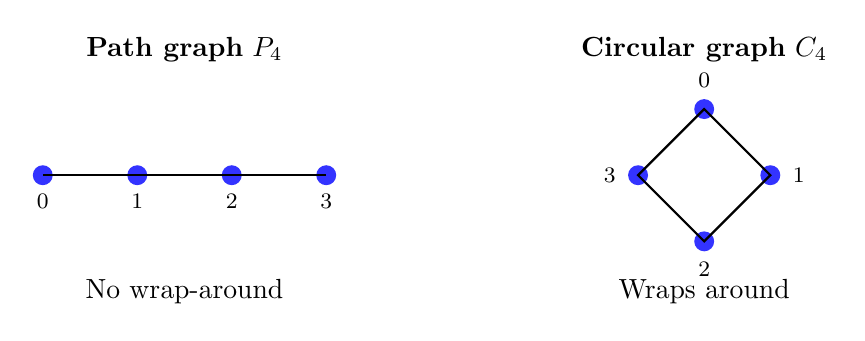
\begin{tikzpicture}[scale=1.2]
    % Path graph
    \node[above] at (1.5, 1.1) {\textbf{Path graph} $P_4$};
    \foreach \i in {0,...,3} {
        \fill[blue!80] (\i, 0) circle (3pt);
        \node[below] at (\i, -0.1) {\footnotesize $\i$};
    }
    \draw[thick] (0,0) -- (1,0) -- (2,0) -- (3,0);
    \node[below] at (1.5, -1) {No wrap-around};
    
    % Circular graph
    \node[above] at (7, 1.1) {\textbf{Circular graph} $C_4$};
    \foreach \i in {0,...,3} {
        \pgfmathsetmacro{\angle}{90 - \i*90}
        \fill[blue!80] ({7 + 0.7*cos(\angle)}, {0.7*sin(\angle)}) circle (3pt);
        \node at ({7 + 1.0*cos(\angle)}, {1.0*sin(\angle)}) {\footnotesize $\i$};
    }
    \draw[thick] ({7 + 0.7*cos(90)}, {0.7*sin(90)}) -- 
                 ({7 + 0.7*cos(0)}, {0.7*sin(0)}) -- 
                 ({7 + 0.7*cos(-90)}, {0.7*sin(-90)}) -- 
                 ({7 + 0.7*cos(180)}, {0.7*sin(180)}) -- cycle;
    \node[below] at (7, -1) {Wraps around};
\end{tikzpicture}
\end{center}

The Laplacians are different:
\[
L_{\text{path}} = \begin{pmatrix}
1 & -1 & 0 & 0 \\
-1 & 2 & -1 & 0 \\
0 & -1 & 2 & -1 \\
0 & 0 & -1 & 1
\end{pmatrix}
\quad \text{vs} \quad
L_{\text{circle}} = \begin{pmatrix}
2 & -1 & 0 & -1 \\
-1 & 2 & -1 & 0 \\
0 & -1 & 2 & -1 \\
-1 & 0 & -1 & 2
\end{pmatrix}
\]

Key differences:
\begin{itemize}
    \item Path: endpoints have degree 1, interior nodes have degree 2
    \item Circle: all nodes have degree 2 (perfect symmetry)
\end{itemize}

\textbf{Consequence}: The eigenvectors of the path graph are 
\emph{not} complex exponentials. They are related to the 
\textbf{Discrete Cosine Transform (DCT)}, not the DFT:
\[
u_k[n] \propto \cos\left(\frac{\pi k (n + \frac{1}{2})}{N}\right)
\]

The boundary conditions fundamentally change the eigenvectors! See 
Appendix~\ref{dft-to-gnn:app:dct-path} for a detailed derivation.
\end{example}

\subsection{Directed Graphs: Symmetry Breaks Down}

A more serious limitation arises with directed graphs.

\begin{definition}[Directed Graph]
In a \textbf{directed graph}, edges have direction: an edge from $i$ 
to $j$ does not imply an edge from $j$ to $i$. The adjacency matrix 
satisfies $A_{ij} \neq A_{ji}$ in general.
\end{definition}

\begin{figure}[H]
\centering
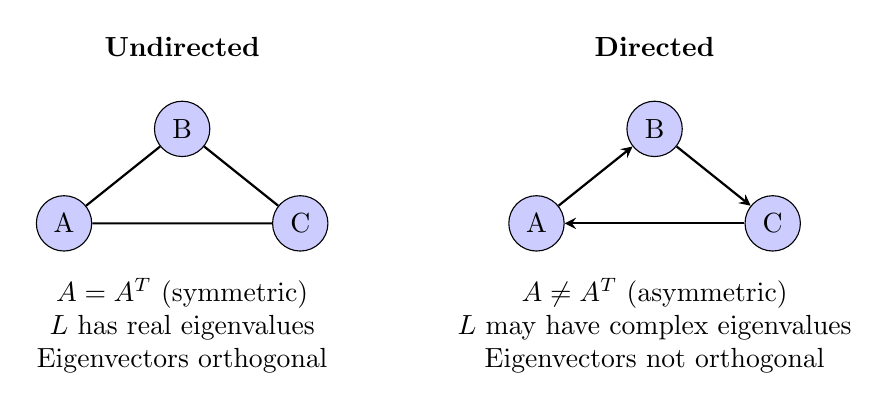
\begin{tikzpicture}[scale=1.0,
    node/.style={circle, draw, fill=blue!20, minimum size=20pt},
    arrow/.style={->, >=stealth, thick}]
    
    % Undirected graph
    \node[above] at (1.5, 2) {\textbf{Undirected}};
    \node[node] (a1) at (0, 0) {A};
    \node[node] (b1) at (1.5, 1.2) {B};
    \node[node] (c1) at (3, 0) {C};
    \draw[thick] (a1) -- (b1) -- (c1) -- (a1);
    
    \node[align=center] at (1.5, -1.3) {$A = A^T$ (symmetric)\\
          $L$ has real eigenvalues\\
          Eigenvectors orthogonal};
    
    % Directed graph
    \node[above] at (7.5, 2) {\textbf{Directed}};
    \node[node] (a2) at (6, 0) {A};
    \node[node] (b2) at (7.5, 1.2) {B};
    \node[node] (c2) at (9, 0) {C};
    \draw[arrow] (a2) -- (b2);
    \draw[arrow] (b2) -- (c2);
    \draw[arrow] (c2) -- (a2);
    
    \node[align=center] at (7.5, -1.3) {$A \neq A^T$ (asymmetric)\\
          $L$ may have complex eigenvalues\\
          Eigenvectors not orthogonal};
\end{tikzpicture}
\caption{Directed graphs break the symmetry that spectral methods 
         rely on.}
\end{figure}

For directed graphs:
\begin{enumerate}
    \item The Laplacian $L = D - A$ is \textbf{not symmetric}
    \item Eigenvalues can be \textbf{complex numbers}
    \item Eigenvectors are \textbf{not orthogonal} (left and right 
          eigenvectors differ)
    \item The matrix may not even be \textbf{diagonalizable}
\end{enumerate}

This breaks the entire spectral framework:
\begin{itemize}
    \item No real "frequencies" to interpret
    \item No orthonormal basis for a "Fourier transform"
    \item The quadratic form $\mathbf{x}^T L \mathbf{x}$ loses its 
          meaning as "smoothness"
\end{itemize}

\begin{example}[A Simple Directed Graph]
Consider a directed 3-cycle: $0 \to 1 \to 2 \to 0$.

\begin{center}
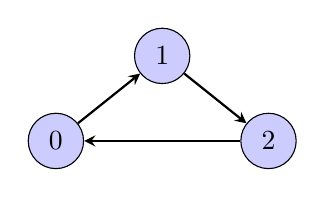
\begin{tikzpicture}[scale=0.9,
    node/.style={circle, draw, fill=blue!20, minimum size=20pt},
    arrow/.style={->, >=stealth, thick}]
    \node[node] (n0) at (0, 0) {0};
    \node[node] (n1) at (1.5, 1.2) {1};
    \node[node] (n2) at (3, 0) {2};
    \draw[arrow] (n0) -- (n1);
    \draw[arrow] (n1) -- (n2);
    \draw[arrow] (n2) -- (n0);
\end{tikzpicture}
\end{center}

\[
A = \begin{pmatrix}
0 & 1 & 0 \\
0 & 0 & 1 \\
1 & 0 & 0
\end{pmatrix}, \quad
D = \begin{pmatrix}
1 & 0 & 0 \\
0 & 1 & 0 \\
0 & 0 & 1
\end{pmatrix}, \quad
L = D - A = \begin{pmatrix}
1 & -1 & 0 \\
0 & 1 & -1 \\
-1 & 0 & 1
\end{pmatrix}
\]

The eigenvalues of $L$ are:
\[
\lambda = 0, \quad \frac{3}{2} + \frac{\sqrt{3}}{2}i, \quad 
\frac{3}{2} - \frac{\sqrt{3}}{2}i
\]

Two of them are \textbf{complex}! There's no meaningful "frequency 
interpretation" for complex eigenvalues in this context.
\end{example}

\subsection{Approaches for Directed Graphs}

Several approaches exist, but none are as clean as the undirected case:

\begin{enumerate}
    \item \textbf{Symmetrization}: Replace $A$ with 
          $\frac{1}{2}(A + A^T)$
          
          \textit{Problem}: Loses directional information entirely
          
    \item \textbf{Magnetic Laplacian}: Encode direction as complex 
          phases $e^{i\theta_{ij}}$ on edges, keeping the matrix 
          Hermitian
          
          \textit{Advantage}: Eigenvalues stay real
          
          \textit{Problem}: How to choose the phases $\theta_{ij}$?
          
    \item \textbf{Random walk Laplacian}: Use $L_{rw} = I - D^{-1}A$
    
          \textit{Problem}: Still not symmetric
          
    \item \textbf{Abandon spectral methods}: Use spatial/message-passing 
          approaches instead (see next section)
\end{enumerate}

\subsection{Computational Cost}

Even for undirected graphs, spectral methods have a practical problem:

\begin{center}
\begin{tabular}{lcc}
\toprule
\textbf{Operation} & \textbf{Spectral} & \textbf{Spatial (1-hop)} \\
\midrule
Eigendecomposition of $L$ & $O(N^3)$ & Not needed \\
Storing eigenvectors $U$ & $O(N^2)$ & Not needed \\
One convolution layer & $O(N^2)$ & $O(|E|)$ \\
\bottomrule
\end{tabular}
\end{center}

For large graphs (social networks with millions of nodes), $O(N^3)$ 
eigendecomposition is completely infeasible. This motivated polynomial 
approximations (ChebNet, GCN), but these are really \emph{spatial} 
methods in disguise---they aggregate information from neighbors without 
ever computing eigenvectors.

%==========================================================================
\section{Message Passing: The General Framework}
%==========================================================================

Given the limitations of spectral methods, we now introduce 
\textbf{message passing} \cite{dft-to-gnn:gilmer2017neural}---a more general framework 
that works on any graph, including directed and heterogeneous graphs.

\subsection{The Key Insight}

The polynomial approximations (ChebNet, GCN) suggest a pattern: instead 
of working in the spectral domain, we can directly aggregate information 
from neighbors. This is the essence of \textbf{spatial} or 
\textbf{message passing} methods.

\begin{center}
\fbox{\parbox{0.9\textwidth}{
\textbf{Message Passing Idea}: Instead of transforming to a global 
frequency domain, each node collects information from its local 
neighborhood and updates its representation accordingly.
}}
\end{center}

\subsection{The Message Passing Paradigm}

\begin{definition}[Message Passing Neural Network]
A \textbf{Message Passing Neural Network (MPNN)} updates node 
representations through three steps:

\begin{enumerate}
    \item \textbf{Message}: Each neighbor $j$ creates a message to send 
          to node $i$
    \item \textbf{Aggregate}: Node $i$ aggregates all incoming messages
    \item \textbf{Update}: Node $i$ updates its representation based on 
          the aggregated messages
\end{enumerate}

Formally, for node $i$ at layer $l$:
\begin{equation}
\boxed{
h_i^{(l+1)} = \phi\left( h_i^{(l)}, 
    \bigoplus_{j \in \mathcal{N}(i)} \psi(h_i^{(l)}, h_j^{(l)}, e_{ji}) 
    \right)
}
\end{equation}
where:
\begin{itemize}
    \item $h_i^{(l)}$ = representation of node $i$ at layer $l$
    \item $\mathcal{N}(i)$ = neighbors of node $i$ (can be in-neighbors 
          for directed graphs)
    \item $\psi$ = \textbf{message function} (creates messages)
    \item $\bigoplus$ = \textbf{aggregation function} (sum, mean, max, 
          attention, ...)
    \item $\phi$ = \textbf{update function} (combines old state with 
          aggregated messages)
    \item $e_{ji}$ = edge features from $j$ to $i$ (optional)
\end{itemize}
\end{definition}

\begin{figure}[H]
\centering
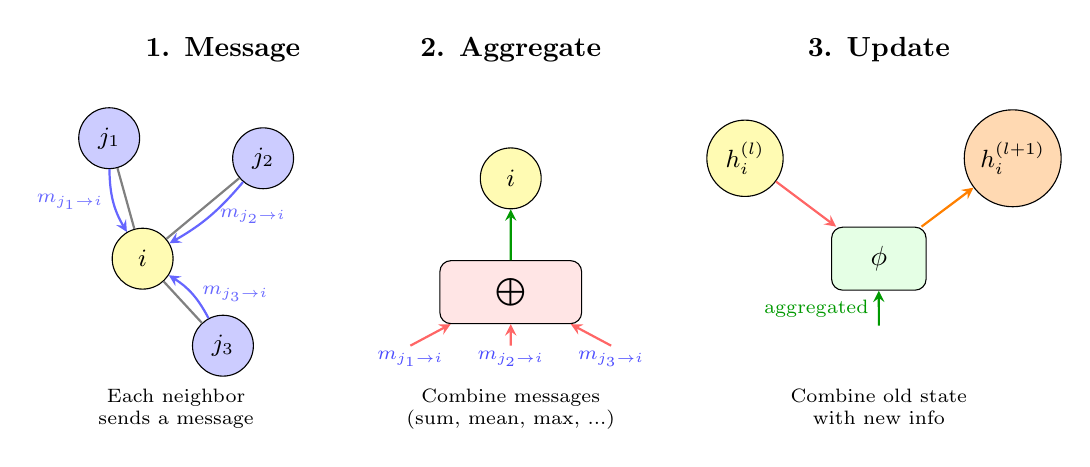
\begin{tikzpicture}[scale=0.85,
    node/.style={circle, draw, minimum size=22pt, font=\small},
    msg/.style={->, >=stealth, thick, blue!60},
    agg/.style={->, >=stealth, thick, red!60}]
    
    % Step 1: Message
    \node[above, font=\bfseries] at (1.2, 2.8) {1. Message};
    \node[node, fill=yellow!30] (a1) at (0, 0) {$i$};
    \node[node, fill=blue!20] (b1) at (-0.5, 1.8) {$j_1$};
    \node[node, fill=blue!20] (c1) at (1.8, 1.5) {$j_2$};
    \node[node, fill=blue!20] (d1) at (1.2, -1.3) {$j_3$};
    
    \draw[thick, gray] (a1) -- (b1);
    \draw[thick, gray] (a1) -- (c1);
    \draw[thick, gray] (a1) -- (d1);
    
    \draw[msg, bend right=15] (b1) to 
        node[left, font=\scriptsize] {$m_{j_1 \to i}$} (a1);
    \draw[msg, bend left=10] (c1) to 
        node[right, font=\scriptsize] {$m_{j_2 \to i}$} (a1);
    \draw[msg, bend right=15] (d1) to 
        node[right, font=\scriptsize] {$m_{j_3 \to i}$} (a1);
    
    \node[below, font=\scriptsize, align=center] at (0.5, -1.8) 
        {Each neighbor\\sends a message};
    
    % Step 2: Aggregate
    \node[above, font=\bfseries] at (5.5, 2.8) {2. Aggregate};
    \node[node, fill=yellow!30] (a2) at (5.5, 1.2) {$i$};
    \node[draw, rounded corners, fill=red!10, 
          minimum width=1.8cm, minimum height=0.8cm] 
        (agg) at (5.5, -0.5) {$\bigoplus$};
    
    \node[font=\scriptsize, blue!70] at (4.0, -1.5) {$m_{j_1 \to i}$};
    \node[font=\scriptsize, blue!70] at (5.5, -1.5) {$m_{j_2 \to i}$};
    \node[font=\scriptsize, blue!70] at (7.0, -1.5) {$m_{j_3 \to i}$};
    
    \draw[agg] (4.0, -1.3) -- (agg);
    \draw[agg] (5.5, -1.3) -- (agg);
    \draw[agg] (7.0, -1.3) -- (agg);
    \draw[agg, green!60!black, thick] (agg) -- (a2);
    
    \node[below, font=\scriptsize, align=center] at (5.5, -1.8) 
        {Combine messages\\(sum, mean, max, ...)};
    
    % Step 3: Update
    \node[above, font=\bfseries] at (11, 2.8) {3. Update};
    \node[node, fill=yellow!30] (a3old) at (9, 1.5) {$h_i^{(l)}$};
    \node[draw, rounded corners, fill=green!10, 
          minimum width=1.2cm, minimum height=0.8cm] 
        (upd) at (11, 0.0) {$\phi$};
    \node[node, fill=orange!30] (a3new) at (13, 1.5) {$h_i^{(l+1)}$};
    
    \draw[agg] (a3old) -- (upd);
    \draw[agg, green!60!black] (11, -1.0) -- (upd) 
        node[left, midway, font=\scriptsize] {aggregated};
    \draw[agg, orange] (upd) -- (a3new);
    
    \node[below, font=\scriptsize, align=center] at (11, -1.8) 
        {Combine old state\\with new info};
    
\end{tikzpicture}
\caption{The three steps of message passing: (1) neighbors create 
         messages, (2) messages are aggregated, (3) node updates 
         its representation.}
\end{figure}

\subsection{Why Message Passing is More General}

Message passing has several advantages over spectral methods:

\begin{center}
\begin{tabular}{lcc}
\toprule
\textbf{Property} & \textbf{Spectral} & \textbf{Message Passing} \\
\midrule
Directed graphs & \color{red}\ding{55} & \color{green!60!black}\ding{51} \\
Edge features & \color{red}\ding{55} & \color{green!60!black}\ding{51} \\
Node-specific transforms & \color{red}\ding{55} & 
    \color{green!60!black}\ding{51} \\
Heterogeneous graphs & \color{red}\ding{55} & 
    \color{green!60!black}\ding{51} \\
Scalability & $O(N^3)$ or $O(N^2)$ & $O(|E|)$ \\
Inductive learning & \color{red}\ding{55} & 
    \color{green!60!black}\ding{51} \\
\bottomrule
\end{tabular}
\end{center}

\textbf{Inductive learning} deserves special mention: spectral methods 
require the eigenvectors $U$, which are specific to a particular graph. 
If the graph changes (new nodes added), we must recompute $U$. Message 
passing methods learn local rules that generalize to new, unseen graphs.

\subsection{Three Flavours of GNN Layers}

The vast majority of GNN architectures can be categorized into three 
"flavours" based on how they compute messages from neighbors 
\cite{dft-to-gnn:bronstein2021geometric}:

\begin{figure}[H]
\centering
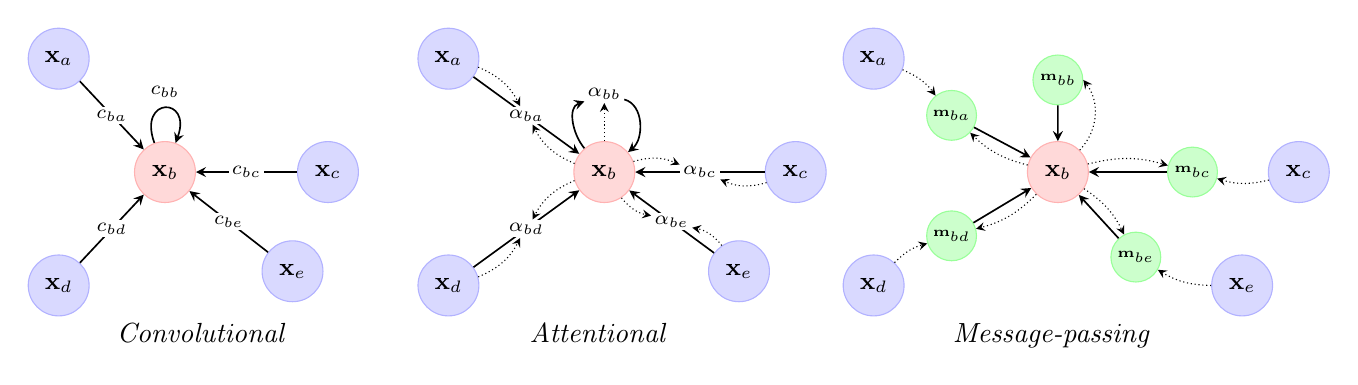
\begin{tikzpicture}[scale=0.9,
    node/.style={circle, draw=blue!30, fill=blue!15, minimum size=22pt,
    font=\bfseries\small, inner sep=1pt},
    centernode/.style={circle, draw=red!30, fill=red!15, minimum size=22pt,
    font=\bfseries\small, inner sep=1pt},
    msgnode/.style={circle, draw=green!40, fill=green!20, minimum size=18pt,
    font=\bfseries\tiny, inner sep=0.5pt},
    arrow/.style={->, >=stealth, semithick},
    dottedarrow/.style={->, >=stealth, thin, densely dotted},
    labelstyle/.style={font=\scriptsize, fill=white, inner sep=1pt}]
    
    % ========== Convolutional ==========
    \begin{scope}[shift={(0,0)}]
        \node[centernode] (b1) at (0, 1.2) {$\mathbf{x}_b$};
        \node[node] (a1) at (-1.5, 2.8) {$\mathbf{x}_a$};
        \node[node] (c1) at (2.3, 1.2) {$\mathbf{x}_c$};
        \node[node] (d1) at (-1.5, -0.4) {$\mathbf{x}_d$};
        \node[node] (e1) at (1.8, -0.2) {$\mathbf{x}_e$};
        
        \foreach \n/\lbl in {a1/c_{ba}, c1/c_{bc}, d1/c_{bd}, e1/c_{be}}
            \draw[arrow] (\n) -- (b1) node[midway, labelstyle] {$\lbl$};
            
        \draw[arrow] (b1) to[out=110, in=70, looseness=6] node[above, font=\scriptsize] {$c_{bb}$} (b1);
        \node[below] at (0.5, -0.8) {\itshape Convolutional};
    \end{scope}
    
    % ========== Attentional ==========
    \begin{scope}[shift={(5,0)}]
        \node[centernode] (b2) at (1.2, 1.2) {$\mathbf{x}_b$};
        \node[node] (a2) at (-1, 2.8) {$\mathbf{x}_a$};
        \node[node] (c2) at (3.9, 1.2) {$\mathbf{x}_c$};
        \node[node] (d2) at (-1, -0.4) {$\mathbf{x}_d$};
        \node[node] (e2) at (3.1, -0.2) {$\mathbf{x}_e$};
        
        \foreach \n/\lbl/\bndS/\bndN in {a2/\alpha_{ba}/20/20, c2/\alpha_{bc}/20/20, d2/\alpha_{bd}/-20/-20, e2/\alpha_{be}/-20/-20} {
            % Main flow arrow
            \draw[arrow] (\n) -- (b2) node (L-\n) [midway, labelstyle] {$\lbl$};
            % Dotted dependencies: from neighbor to alpha, and from center to alpha
            \draw[dottedarrow] (\n) to[bend left={\bndN}] (L-\n);
            \draw[dottedarrow] (b2) to[bend left={\bndS}] (L-\n);
        }
        
        % Self-loop with dependency
        \node (L-bb) at (1.2, 2.3) [labelstyle] {$\alpha_{bb}$};
        \draw[arrow] (b2) to[out=130, in=200, looseness=1] (L-bb);
        \draw[arrow] (L-bb) to[out=-15, in=40, looseness=1] (b2);
        \draw[dottedarrow] (b2) -- (L-bb);
        
        \node[below] at (1.1, -0.8) {\itshape Attentional};
    \end{scope}
    
    % ========== Message-passing ==========
    \begin{scope}[shift={(10,0)}]
        \node[centernode] (b3) at (2.6, 1.2) {$\mathbf{x}_b$};
        \node[node] (a3) at (0, 2.8) {$\mathbf{x}_a$};
        \node[node] (c3) at (6, 1.2) {$\mathbf{x}_c$};
        \node[node] (d3) at (0, -0.4) {$\mathbf{x}_d$};
        \node[node] (e3) at (5.2, -0.4) {$\mathbf{x}_e$};
        
        \node[msgnode] (ma) at (1.1, 2.0) {$\mathbf{m}_{ba}$};
        \node[msgnode] (mc) at (4.5, 1.2) {$\mathbf{m}_{bc}$};
        \node[msgnode] (md) at (1.1, 0.3) {$\mathbf{m}_{bd}$};
        \node[msgnode] (me) at (3.7, 0) {$\mathbf{m}_{be}$};
        \node[msgnode] (mb) at (2.6, 2.5) {$\mathbf{m}_{bb}$};
        
        \foreach \m/\src in {ma/a3, mc/c3, md/d3, me/e3} {
            \draw[arrow] (\m) -- (b3);
            \draw[dottedarrow] (\src) to[bend left=15] (\m);
            \draw[dottedarrow] (b3) to[bend left=15] (\m);
        }
        
        \draw[arrow] (mb) -- (b3);
        \draw[dottedarrow] (b3.north east) to[bend right=40] (mb.east);
        
        \node[below] at (2.5, -0.8) {\itshape Message-passing};
    \end{scope}
\end{tikzpicture}
\caption{Three flavours of GNN layers (adapted from \cite{dft-to-gnn:bronstein2021geometric}), 
         showing the dataflow for updating node $b$ from its neighborhood. 
         \textbf{Left}: Convolutional---sender node features are multiplied 
         by constant weights $c_{uv}$ from the graph structure. 
         \textbf{Middle}: Attentional---weights $\alpha_{uv} = a(\mathbf{x}_u, \mathbf{x}_v)$ 
         are implicitly computed via attention (dotted arrows show the 
         receiver attending to senders).
         \textbf{Right}: Message-passing---vector messages 
         $\mathbf{m}_{uv} = \psi(\mathbf{x}_u, \mathbf{x}_v)$ are computed 
         based on both sender and receiver (dotted arrows), then aggregated 
         (solid arrows).}
\label{dft-to-gnn:fig:three-flavours}
\end{figure}


\begin{enumerate}
    \item \textbf{Convolutional} (e.g., GCN): Messages are scaled by 
          fixed coefficients $c_{uv}$ that depend only on graph structure:
          \[
          h_u = \phi\left(x_u, \bigoplus_{v \in \mathcal{N}(u)} c_{uv} \, \psi(x_v)\right)
          \]
          
    \item \textbf{Attentional} (e.g., GAT): Coefficients are computed 
          dynamically via an attention mechanism:
          \[
          h_u = \phi\left(x_u, \bigoplus_{v \in \mathcal{N}(u)} 
              a(x_u, x_v) \, \psi(x_v)\right)
          \]
          
    \item \textbf{Message-passing} (general): Full vector messages are 
          computed based on both sender and receiver:
          \[
          h_u = \phi\left(x_u, \bigoplus_{v \in \mathcal{N}(u)} 
              \psi(x_u, x_v)\right)
          \]
\end{enumerate}

These form a hierarchy of expressiveness: 
\textbf{convolutional $\subset$ attentional $\subset$ message-passing}. 
Attentional GNNs can represent convolutional GNNs by setting 
$a(x_u, x_v) = c_{uv}$, and message-passing generalizes both by allowing 
vector-valued (rather than scalar) interactions between nodes.

\subsection{Example: GCN as Message Passing}

Let's see how the GCN layer fits into the message passing framework.

\begin{example}[GCN Layer]
Recall from Section~8 that the GCN layer in matrix form is:
\[
H^{(l+1)} = \sigma\left( \hat{D}^{-1/2} \hat{A} \hat{D}^{-1/2} 
             H^{(l)} W^{(l)} \right)
\]
where $\hat{A} = A + I$ (adjacency with self-loops), $\hat{D}$ is 
its degree matrix, and $H^{(l)} \in \mathbb{R}^{N \times d}$ has node 
features as rows.

\textbf{Deriving the per-node form.} The $(i,j)$ entry of 
$\hat{D}^{-1/2} \hat{A} \hat{D}^{-1/2}$ is:
\[
\left(\hat{D}^{-1/2} \hat{A} \hat{D}^{-1/2}\right)_{ij} = 
\frac{\hat{A}_{ij}}{\sqrt{\hat{d}_i}\sqrt{\hat{d}_j}}
\]
where $\hat{d}_i = d_i + 1$ is the degree including the self-loop.

Since $\hat{A}_{ij} = 1$ if $j \in \mathcal{N}(i) \cup \{i\}$ and $0$ 
otherwise, the $i$-th row of $\hat{D}^{-1/2} \hat{A} \hat{D}^{-1/2} H^{(l)}$ is:
\[
\sum_{j \in \mathcal{N}(i) \cup \{i\}} 
    \frac{1}{\sqrt{\hat{d}_i}\sqrt{\hat{d}_j}} h_j^{(l)}
\]
where $h_j^{(l)}$ is the $j$-th row of $H^{(l)}$ (a row vector).

Multiplying by $W^{(l)}$ on the right and applying $\sigma$, the 
updated feature vector for node $i$ is:
\[
h_i^{(l+1)} = \sigma\left( \sum_{j \in \mathcal{N}(i) \cup \{i\}} 
    \frac{1}{\sqrt{d_i + 1}\sqrt{d_j + 1}} h_j^{(l)} W^{(l)} \right)
\]

\textbf{In message passing terms:}
\begin{itemize}
    \item \textbf{Message from $j$ to $i$}: 
          $m_{j \to i} = \frac{1}{\sqrt{d_i+1}\sqrt{d_j+1}} h_j W$
    \item \textbf{Aggregation}: $\bigoplus = \sum$ (summation)
    \item \textbf{Update}: $\phi = \sigma$ (nonlinearity, e.g., ReLU)
\end{itemize}

The normalization $\frac{1}{\sqrt{d_i+1}\sqrt{d_j+1}}$ comes from the 
symmetric normalized adjacency and prevents high-degree nodes from 
dominating the aggregation.
\end{example}

\subsection{Example: GraphSAGE}

GraphSAGE \cite{dft-to-gnn:hamilton2017inductive} (Sample and Aggregate) is a popular message passing variant:

\begin{example}[GraphSAGE Layer]
\[
h_i^{(l+1)} = \sigma\left( 
    \text{CONCAT}\left( 
    h_i^{(l)}, \text{AGG}(\{h_j^{(l)} : j \in \mathcal{N}(i)\}) 
    \right) W^{(l)} \right)
\]

Key features:
\begin{itemize}
    \item \textbf{Message}: Identity (just use neighbor features)
    \item \textbf{Aggregation}: Mean, max-pooling, or LSTM
    \item \textbf{Update}: Concatenate self with aggregated neighbors, 
          then linear transform by $W$
\end{itemize}

The concatenation explicitly separates "self" information from 
"neighbor" information.
\end{example}

\subsection{Example: Graph Attention Networks (GAT)}

GAT \cite{dft-to-gnn:velickovic2018graph} introduces learnable attention weights:

\begin{example}[GAT Layer]
\[
h_i^{(l+1)} = \sigma\left( \sum_{j \in \mathcal{N}(i) \cup \{i\}} 
    \alpha_{ij} \, h_j^{(l)} W \right)
\]

where the attention coefficients $\alpha_{ij}$ are computed as:
\[
\alpha_{ij} = \frac{\exp\bigl(\text{LeakyReLU}(
    [h_i W \| h_j W] \, \mathbf{a})\bigr)}
    {\sum_{k \in \mathcal{N}(i) \cup \{i\}} \exp\bigl(\text{LeakyReLU}(
    [h_i W \| h_k W] \, \mathbf{a})\bigr)}
\]

Here $[h_i W \| h_j W]$ denotes concatenation of the two transformed 
row vectors (giving a row vector of size $2d'$), and 
$\mathbf{a} \in \mathbb{R}^{2d'}$ is a learnable attention vector.

Key features:
\begin{itemize}
    \item \textbf{Message}: Weighted by learned attention $\alpha_{ij}$
    \item \textbf{Aggregation}: Weighted sum (attention-based)
    \item The network \emph{learns} which neighbors are important
\end{itemize}
\end{example}

\subsection{Spectral Convolution as a Special Case of Message Passing}

Here's the key insight that unifies everything:

\begin{theorem}[Spectral Convolution is Message Passing]
Any polynomial spectral filter $g(L) = \sum_{k=0}^{K} \theta_k L^k$ 
can be written as $K$ rounds of message passing.
\end{theorem}

\begin{proof}[Proof sketch]
The key observation is that $L\mathbf{x}$ is a local operation:
\[
(L\mathbf{x})_i = d_i x_i - \sum_{j \in \mathcal{N}(i)} x_j 
    = \sum_{j \in \mathcal{N}(i)} (x_i - x_j)
\]

This only involves node $i$ and its immediate neighbors---it's one 
round of message passing!

Similarly, $L^2 \mathbf{x} = L(L\mathbf{x})$ involves 2-hop neighbors, 
$L^3 \mathbf{x}$ involves 3-hop neighbors, and so on.

Therefore, $g(L)\mathbf{x} = \sum_{k=0}^{K} \theta_k L^k \mathbf{x}$ 
aggregates information from up to $K$-hop neighbors, which is exactly 
what $K$ rounds of message passing does.
\end{proof}

\begin{figure}[H]
\centering
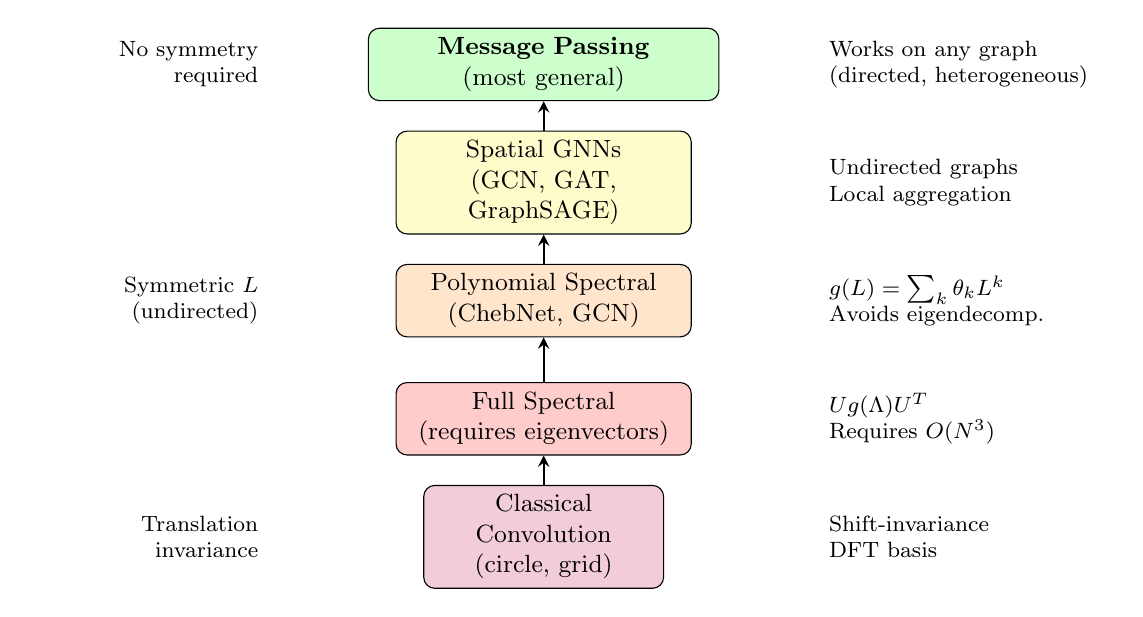
\begin{tikzpicture}[
    concept/.style={rectangle, draw, rounded corners, fill=blue!10, 
                    text width=7em, minimum height=2.5em, 
                    text centered, font=\small},
    arrow/.style={->, >=stealth, thick}
]

% Hierarchy
\node[concept, fill=green!20, text width=12em] (mp) at (0, 3) 
    {\textbf{Message Passing}\\(most general)};

\node[concept, fill=yellow!20, text width=10em] (spatial) at (0, 1.5) 
    {Spatial GNNs\\(GCN, GAT, GraphSAGE)};

\node[concept, fill=orange!20, text width=10em] (poly) at (0, 0) 
    {Polynomial Spectral\\(ChebNet, GCN)};

\node[concept, fill=red!20, text width=10em] (spectral) at (0, -1.5) 
    {Full Spectral\\(requires eigenvectors)};

\node[concept, fill=purple!20, text width=8em] (classical) at (0, -3) 
    {Classical Convolution\\(circle, grid)};

% Arrows showing "special case of"
\draw[arrow] (spatial) -- (mp);
\draw[arrow] (poly) -- (spatial);
\draw[arrow] (spectral) -- (poly);
\draw[arrow] (classical) -- (spectral);

% Annotations
\node[right, font=\footnotesize, text width=10em] at (3.5, 3) 
    {Works on any graph\\(directed, heterogeneous)};
\node[right, font=\footnotesize, text width=10em] at (3.5, 1.5) 
    {Undirected graphs\\Local aggregation};
\node[right, font=\footnotesize, text width=10em] at (3.5, 0) 
    {$g(L) = \sum_k \theta_k L^k$\\Avoids eigendecomp.};
\node[right, font=\footnotesize, text width=10em] at (3.5, -1.5) 
    {$U g(\Lambda) U^T$\\Requires $O(N^3)$};
\node[right, font=\footnotesize, text width=10em] at (3.5, -3) 
    {Shift-invariance\\DFT basis};

% Left annotations - requirements
\node[left, font=\footnotesize, text width=8em, align=right] at (-3.5, 3) 
    {No symmetry\\required};
\node[left, font=\footnotesize, text width=8em, align=right] at (-3.5, 0) 
    {Symmetric $L$\\(undirected)};
\node[left, font=\footnotesize, text width=8em, align=right] at (-3.5, -3) 
    {Translation\\invariance};

\end{tikzpicture}
\caption{The hierarchy of graph neural network methods. Each level is 
         a special case of the one above. Message passing is the most 
         general framework.}
\label{dft-to-gnn:fig:hierarchy}
\end{figure}

\subsection{When to Use Which Approach}

\begin{itemize}
    \item \textbf{Full spectral methods}: Rarely used in practice due 
          to $O(N^3)$ cost. Useful for theoretical analysis and small 
          graphs.
    
    \item \textbf{Polynomial spectral (ChebNet, GCN)}: Good balance of 
          theory and practice. The spectral interpretation helps 
          understand what the network learns (low-pass vs high-pass 
          filters).
    
    \item \textbf{General message passing (GAT, GraphSAGE)}: Most 
          flexible. Use when you have directed graphs, edge features, 
          heterogeneous node types, or need inductive learning (applying 
          to new graphs).
\end{itemize}

\begin{remark}[The Value of the Spectral Perspective]
Even though message passing is more general and practical, the spectral 
perspective remains valuable:

\begin{enumerate}
    \item It explains \emph{why} GNNs work as frequency filters
    \item It helps understand \textbf{over-smoothing}: too many layers 
          $\approx$ low-pass filter that kills all signal
    \item It provides design principles: if you want to preserve 
          high-frequency information, design filters accordingly
    \item It connects to classical signal processing intuition
\end{enumerate}

The spectral view is for \emph{understanding}; message passing is for 
\emph{implementation}.
\end{remark}

%==========================================================================
\section{Summary and Key Takeaways}
%==========================================================================

\subsection{What We've Learned}

\begin{enumerate}
\item \textbf{The DFT has geometric meaning}: It expresses a signal in 
      the eigenbasis of the circular graph Laplacian. The DFT basis 
      vectors are forced by the circular symmetry.

\item \textbf{The convolution theorem has a deep explanation}: 
      Circulant matrices (which represent \textbf{circular} convolution 
      on the circle) are all diagonalized by the same eigenvectors---the 
      DFT basis. This is why convolution becomes multiplication.

\item \textbf{Linear vs Circular Convolution}: The DFT naturally gives 
      circular convolution; linear convolution requires zero-padding to 
      avoid wrap-around effects. Zero-padding creates a "buffer zone" 
      that prevents interference between periods.

\item \textbf{Generalization to graphs}: The Graph Fourier Transform 
      uses Laplacian eigenvectors as a frequency basis. But this is a 
      \emph{definition by analogy}, not a theorem---general graphs lack 
      the shift-invariance that makes the circular case special.

\item \textbf{Spectral methods have limitations}: They require symmetric 
      (undirected) graphs, expensive $O(N^3)$ eigendecomposition, and 
      cannot handle edge features or heterogeneous graphs.

\item \textbf{Message passing is the general framework}: It works on 
      any graph (directed, heterogeneous) and scales as $O(|E|)$. 
      Spectral convolution is a special case of message passing.

\item \textbf{The hierarchy}: Classical convolution $\subset$ Spectral 
      graph convolution $\subset$ Polynomial filters $\subset$ Spatial 
      GNNs $\subset$ Message passing.

\item \textbf{Theory vs Practice}: The spectral view provides 
      theoretical understanding (frequency filtering, over-smoothing); 
      message passing provides practical implementation.
\end{enumerate}

\subsection{Key Formulas}

\begin{center}
\renewcommand{\arraystretch}{1.6}
\begin{tabular}{ll}
\toprule
\textbf{Concept} & \textbf{Formula} \\
\midrule
DFT & $X_k = \sum_{n=0}^{N-1} x_n \, e^{-2\pi i kn/N}$ \\[0.3em]
Inverse DFT & $x_n = \frac{1}{N} \sum_{k=0}^{N-1} X_k \, 
              e^{2\pi i kn/N}$ \\[0.3em]
Circular Convolution & $y_n = \sum_{m=0}^{N-1} x_m h_{(n-m) \mod N}$ \\[0.3em]
Circular Conv.\ Theorem & $\text{DFT}(\mathbf{x} \circledast \mathbf{h}) 
                         = \text{DFT}(\mathbf{x}) \odot 
                           \text{DFT}(\mathbf{h})$ \\[0.3em]
Linear Conv.\ via DFT & Zero-pad to $L \geq N+M-1$, then use circular \\[0.3em]
Graph Laplacian & $L = D - A$ \\[0.3em]
Graph Fourier Transform & $\hat{\mathbf{x}} = U^T \mathbf{x}$ where 
                          $L = U\Lambda U^T$ \\[0.3em]
Spectral Graph Conv.\ & $\mathbf{x} *_G g 
                        = U \, g(\Lambda) \, U^T \mathbf{x}$ \\[0.3em]
Message Passing & $h_i^{(l+1)} = \phi\bigl( h_i^{(l)}, 
                  \bigoplus_{j \in \mathcal{N}(i)} 
                  \psi(h_i^{(l)}, h_j^{(l)}, e_{ji}) \bigr)$ \\[0.3em]
GCN Layer & $H^{(l+1)} = \sigma(\tilde{D}^{-1/2}\tilde{A}
            \tilde{D}^{-1/2} H^{(l)} W^{(l)})$ \\
\bottomrule
\end{tabular}
\end{center}

\subsection{The Big Picture}

\begin{center}
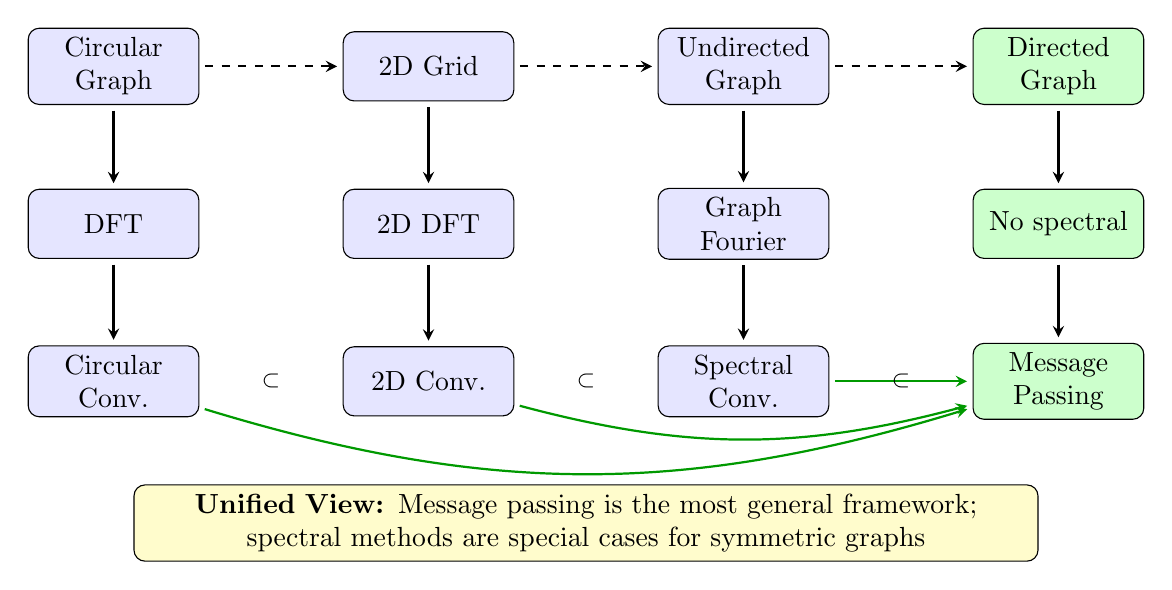
\begin{tikzpicture}[
    concept/.style={rectangle, draw, rounded corners, fill=blue!10, 
                    text width=5.5em, minimum height=2.5em, 
                    text centered},
    arrow/.style={->, >=stealth, thick, shorten >=2pt, shorten <=2pt}
]

% Top row - Graph types
\node[concept] (circle) at (0, 4) {Circular Graph};
\node[concept] (grid) at (4, 4) {2D Grid};
\node[concept] (undirected) at (8, 4) {Undirected Graph};
\node[concept, fill=green!20] (directed) at (12, 4) {Directed Graph};

% Second row - Transforms
\node[concept] (dft) at (0, 2) {DFT};
\node[concept] (dft2d) at (4, 2) {2D DFT};
\node[concept] (gft) at (8, 2) {Graph Fourier};
\node[concept, fill=green!20] (none) at (12, 2) {No spectral};

% Third row - Operations
\node[concept] (conv1d) at (0, 0) {Circular Conv.};
\node[concept] (conv2d) at (4, 0) {2D Conv.};
\node[concept] (gconv) at (8, 0) {Spectral Conv.};
\node[concept, fill=green!20] (mp) at (12, 0) {Message Passing};

% Vertical arrows
\draw[arrow] (circle) -- (dft);
\draw[arrow] (grid) -- (dft2d);
\draw[arrow] (undirected) -- (gft);
\draw[arrow] (directed) -- (none);

\draw[arrow] (dft) -- (conv1d);
\draw[arrow] (dft2d) -- (conv2d);
\draw[arrow] (gft) -- (gconv);
\draw[arrow] (none) -- (mp);

% Horizontal arrows (generalization)
\draw[arrow, dashed] (circle) -- (grid);
\draw[arrow, dashed] (grid) -- (undirected);
\draw[arrow, dashed] (undirected) -- (directed);

% Message passing encompasses all
\draw[arrow, green!60!black, thick] (conv1d) to[bend right=17] (mp);
\draw[arrow, green!60!black, thick] (conv2d) to[bend right=15] (mp);
\draw[arrow, green!60!black, thick] (gconv) -- (mp);

% Labels
\node[font=\footnotesize] at (10, 0) {$\subset$};
\node[font=\footnotesize] at (6, 0) {$\subset$};
\node[font=\footnotesize] at (2, 0) {$\subset$};

% Bottom annotation
\node[draw, rounded corners, fill=yellow!20, text width=32em, 
      minimum height=1.5em, align=center] at (6, -1.8) {
      \textbf{Unified View:} Message passing is the most general 
      framework;\\spectral methods are special cases for symmetric graphs};

\end{tikzpicture}
\end{center}

\begin{remark}[Final Insight]
This document has traced a path from the DFT to modern Graph Neural 
Networks, revealing a beautiful mathematical structure:

\begin{itemize}
\item \textbf{On the circle}: Translation invariance forces complex 
      exponentials as eigenfunctions $\rightarrow$ DFT
\item \textbf{On undirected graphs}: The Laplacian's eigenvectors 
      provide a natural frequency basis $\rightarrow$ Graph Fourier 
      Transform (but this is a definition, not a theorem)
\item \textbf{Limitations}: Directed graphs, computational cost, and 
      lack of true shift-invariance limit spectral methods
\item \textbf{Message passing}: The general framework that encompasses 
      all these special cases while working on any graph
\end{itemize}

The spectral perspective remains invaluable for \emph{understanding}:
it explains why GNNs act as frequency filters, why over-smoothing 
occurs (too many low-pass filters), and connects to classical signal 
processing intuition.

But for \emph{implementation}, message passing is the practical 
workhorse: it's more general, more scalable, and more flexible.

The deep insight is that these are not competing approaches---they're 
different views of the same underlying mathematics. Understanding both 
perspectives makes you a better practitioner: use spectral intuition 
to design architectures, and message passing to implement them.
\end{remark}

%==========================================================================
\newpage
\chapterappendix
\section{Why Complex Exponentials? Translation Invariance}
\label{dft-to-gnn:app:translation-invariance}
%==========================================================================

This appendix provides a detailed proof of why complex exponentials 
are the eigenfunctions of the circular graph Laplacian. The key insight 
is that this is forced by \textbf{translation invariance}.

\subsection{The Fundamental Question}

We showed in Section~3 that the eigenvectors of the circular graph 
Laplacian are complex exponentials $e^{2\pi i kn/N}$. But \emph{why} 
are complex exponentials special? Why not some other basis?

\subsection{Translation Invariance}

A system is \textbf{translation-invariant} (or shift-invariant) if 
shifting the input shifts the output by the same amount. For a discrete 
system on the circle, define the shift operator:
\[
(T_a \mathbf{x})_n = x_{n-a \mod N}
\]
Translation invariance means that for any linear operator $L$:
\[
L T_a = T_a L \quad \text{for all } a
\]

The circular graph Laplacian satisfies this property because every node 
"looks the same" as every other node---the graph has perfect rotational 
symmetry.

\subsection{The Main Theorem}

\begin{theorem}[Exponentials as Forced Eigenfunctions]
\label{dft-to-gnn:thm:app-forced-eigenfunctions}
If an operator $L$ commutes with all circular shifts 
($L T_a = T_a L$ for all $a$), then the eigenfunctions of $L$ must be 
of the form $e^{2\pi i kn/N}$ for integer $k$.
\end{theorem}

\begin{proof}
The proof proceeds in several steps:

\textbf{Step 1: Shifted eigenvectors are still eigenvectors.}

Assume $L\mathbf{v} = \lambda \mathbf{v}$. Apply $T_a$ to both sides:
\[
T_a(L\mathbf{v}) = T_a(\lambda \mathbf{v}) = \lambda (T_a \mathbf{v})
\]
Since $LT_a = T_a L$, we have $T_a(L\mathbf{v}) = L(T_a \mathbf{v})$, so:
\[
L(T_a \mathbf{v}) = \lambda (T_a \mathbf{v})
\]
Thus $T_a \mathbf{v}$ is also an eigenvector with eigenvalue $\lambda$.

\textbf{Step 2: Eigenvectors are scaled by shifts.}

If the eigenspace for $\lambda$ is one-dimensional, then $T_a \mathbf{v}$ 
must be a scalar multiple of $\mathbf{v}$:
\[
T_a \mathbf{v} = \mu(a) \mathbf{v}
\]
for some scalar $\mu(a)$ depending on the shift amount $a$.

\textbf{Step 3: The scaling function is multiplicative.}

The shift operators satisfy the group property $T_a T_b = T_{a+b}$. 
Applying both sides to $\mathbf{v}$:
\[
T_a(T_b \mathbf{v}) = T_a(\mu(b) \mathbf{v}) = \mu(b) \cdot \mu(a) \mathbf{v}
\]
\[
T_{a+b} \mathbf{v} = \mu(a+b) \mathbf{v}
\]
Therefore: $\mu(a+b) = \mu(a) \cdot \mu(b)$

\textbf{Step 4: Solve the functional equation.}

The functional equation $\mu(a+b) = \mu(a)\mu(b)$ with $\mu(0) = 1$ has 
the general solution $\mu(a) = e^{ca}$ for some constant $c$.

\textbf{Step 5: Apply periodicity.}

On a circle of $N$ points, shifting by $N$ returns to the original 
position: $T_N = T_0 = I$. Therefore:
\[
\mu(N) = 1 \quad \Rightarrow \quad e^{cN} = 1 \quad \Rightarrow \quad 
cN = 2\pi i k
\]
for some integer $k$. Thus $c = 2\pi i k/N$ and:
\[
\mu(a) = e^{2\pi i ka/N}
\]

\textbf{Step 6: Derive the eigenvector form.}

From $T_a \mathbf{v} = \mu(a) \mathbf{v}$, we have for each component:
\[
v_{n-a} = e^{2\pi i ka/N} v_n
\]
Setting $m = n - a$ (so $a = n - m$):
\[
v_m = e^{2\pi i k(n-m)/N} v_n = e^{2\pi i kn/N} \cdot e^{-2\pi i km/N} v_n
\]
For this to hold for all $m, n$, we need:
\[
v_m = C \cdot e^{2\pi i km/N}
\]
for some constant $C$. Normalizing gives the standard DFT basis vectors.
\end{proof}

\subsection{The Universal Principle}

This result explains why Fourier analysis appears throughout science:

\begin{center}
\fbox{\parbox{0.9\textwidth}{
\textbf{Any system that is translation-invariant is diagonalized by 
complex exponentials.}
}}
\end{center}

\textbf{Examples:}
\begin{itemize}
\item \textbf{Time-invariant linear systems} (signal processing): 
      Time translation invariance $\Rightarrow$ frequency domain analysis
\item \textbf{Spatially homogeneous media} (wave propagation): 
      Space translation invariance $\Rightarrow$ spatial Fourier transforms
\item \textbf{Crystals with periodic structure} (solid-state physics): 
      Lattice translation invariance $\Rightarrow$ Bloch's theorem
\item \textbf{Stationary random processes} (probability): 
      Time translation invariance $\Rightarrow$ spectral density
\end{itemize}

\subsection{Implications for Graphs}

For general graphs without translational symmetry:
\begin{itemize}
\item The Laplacian does \emph{not} commute with any non-trivial shift
\item Eigenvectors are \emph{not} complex exponentials
\item But the eigenvectors still provide a natural "frequency basis" 
      (ordered by eigenvalue = smoothness)
\end{itemize}

This is why spectral graph convolution \emph{defines} frequency analysis 
using Laplacian eigenvectors, rather than \emph{deriving} it from 
symmetry principles. The circular graph is special precisely because 
it has the translation symmetry that forces the exponential basis.

%==========================================================================
\newpage
\section{The Path Graph and the Discrete Cosine Transform}
\label{dft-to-gnn:app:dct-path}
%==========================================================================

Just as the circular graph leads to the DFT, the \textbf{path graph} 
leads to the \textbf{Discrete Cosine Transform (DCT)}. This appendix 
proves this connection and explains why boundary conditions matter.

\subsection{The Path Graph Laplacian}

The path graph $P_N$ has $N$ nodes connected in a line:
\begin{center}
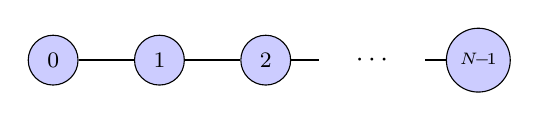
\begin{tikzpicture}[scale=0.9]
    \foreach \i in {0,1,2} {
        \node[circle, draw, fill=blue!20, minimum size=18pt] 
            (n\i) at (\i*1.5, 0) {\footnotesize $\i$};
    }
    \node at (4.5, 0) {$\cdots$};
    \node[circle, draw, fill=blue!20, minimum size=18pt] 
        (nm1) at (6, 0) {\footnotesize $\scriptstyle N\!-\!1$};
    
    \draw[thick] (n0) -- (n1) -- (n2) -- (3.75, 0);
    \draw[thick] (5.25, 0) -- (nm1);
\end{tikzpicture}
\end{center}

Unlike the circular graph, there is \textbf{no edge} from node $N-1$ 
back to node $0$. The Laplacian is:
\[
L_{\text{path}} = \begin{pmatrix}
1 & -1 & 0 & \cdots & 0 \\
-1 & 2 & -1 & \cdots & 0 \\
0 & -1 & 2 & \cdots & 0 \\
\vdots & & \ddots & \ddots & -1 \\
0 & 0 & \cdots & -1 & 1
\end{pmatrix}
\]

Note the \textbf{boundary conditions}: the corner entries are $1$ (not 
$2$) because the endpoints have degree $1$.

\subsection{Finding the Eigenvectors}

For the interior nodes ($1 \leq n \leq N-2$), the eigenvalue equation 
$L\mathbf{u} = \lambda \mathbf{u}$ gives:
\[
-u_{n-1} + 2u_n - u_{n+1} = \lambda u_n
\]

This is the same recurrence as for the circular graph! So we try 
$u_n = e^{i\omega n}$, which gives:
\[
-e^{-i\omega} + 2 - e^{i\omega} = \lambda 
\quad \Rightarrow \quad 
\lambda = 2 - 2\cos\omega = 4\sin^2(\omega/2)
\]

The general solution is $u_n = A e^{i\omega n} + B e^{-i\omega n}$, or 
equivalently:
\[
u_n = C \cos(\omega n) + D \sin(\omega n)
\]

\subsection{Applying Boundary Conditions}

Now we apply the boundary conditions. At $n = 0$:
\[
u_0 - u_1 = \lambda u_0 \quad \Rightarrow \quad 
u_1 = (1 - \lambda) u_0
\]

At $n = N-1$:
\[
-u_{N-2} + u_{N-1} = \lambda u_{N-1} \quad \Rightarrow \quad 
u_{N-2} = (1 - \lambda) u_{N-1}
\]

These are \textbf{Neumann-like} boundary conditions (the discrete 
analog of $\frac{du}{dx} = 0$ at the boundary).

For the ansatz $u_n = C \cos(\omega n + \phi)$, the boundary condition 
at $n = 0$ gives:
\[
\cos\phi - \cos(\omega + \phi) = \lambda \cos\phi
\]

Using $\lambda = 2(1 - \cos\omega)$, this simplifies to:
\[
\cos\phi - \cos(\omega + \phi) = 2(1 - \cos\omega)\cos\phi
\]

After trigonometric manipulation, this is satisfied when 
$\phi = \omega/2$, giving:
\[
u_n = \cos\left(\omega\left(n + \frac{1}{2}\right)\right)
\]

The boundary condition at $n = N-1$ then requires:
\[
\omega \cdot N = k\pi \quad \text{for } k = 0, 1, \ldots, N-1
\]

\subsection{The DCT-II Basis}

Combining these results, the eigenvectors of the path graph are:

\begin{theorem}[Path Graph Eigenvectors = DCT-II Basis]
\label{dft-to-gnn:thm:path-dct}
The eigenvectors of the path graph Laplacian $L_{P_N}$ are:
\begin{equation}
u_k[n] = \sqrt{\frac{2 - \delta_{k0}}{N}} \cos\left(\frac{\pi k (n + \frac{1}{2})}{N}\right), 
\quad k = 0, 1, \ldots, N-1
\end{equation}
with eigenvalues:
\begin{equation}
\lambda_k = 4\sin^2\left(\frac{\pi k}{2N}\right) = 
2\left(1 - \cos\frac{\pi k}{N}\right)
\end{equation}
where $\delta_{k0}$ is the Kronecker delta (the normalization factor 
is $\sqrt{1/N}$ for $k=0$ and $\sqrt{2/N}$ for $k > 0$).
\end{theorem}

These are exactly the basis vectors of the \textbf{DCT-II} (the most 
common DCT variant, often just called "the DCT").

\subsection{Comparison: DFT vs DCT}

\begin{center}
\renewcommand{\arraystretch}{1.4}
\begin{tabular}{lcc}
\toprule
\textbf{Property} & \textbf{DFT (Circular Graph)} & \textbf{DCT (Path Graph)} \\
\midrule
Graph structure & Circle (periodic) & Path (endpoints) \\
Boundary condition & Periodic: $u_{N} = u_0$ & Neumann-like \\
Basis functions & $e^{2\pi i kn/N}$ & $\cos\left(\frac{\pi k(n+1/2)}{N}\right)$ \\
Eigenvalues & $4\sin^2(\pi k/N)$ & $4\sin^2(\pi k/2N)$ \\
Values & Complex & Real \\
Symmetry & Translation invariance & Reflection symmetry \\
\bottomrule
\end{tabular}
\end{center}

\subsection{Why This Matters}

\begin{enumerate}
\item \textbf{Boundary conditions determine the transform.} The same 
      differential operator (second derivative / graph Laplacian) gives 
      different eigenvectors depending on boundary conditions:
      \begin{itemize}
          \item Periodic boundaries $\rightarrow$ DFT (complex exponentials)
          \item Neumann boundaries $\rightarrow$ DCT (cosines)
          \item Dirichlet boundaries ($u = 0$ at endpoints) $\rightarrow$ 
                DST (Discrete Sine Transform)
      \end{itemize}

\item \textbf{The DCT is widely used in practice.} JPEG image compression 
      uses the DCT precisely because images have boundaries (edges) rather 
      than periodic structure. The DCT handles boundaries more naturally 
      than the DFT.

\item \textbf{General graphs have no such structure.} For an arbitrary 
      graph, there's no clean formula for the eigenvectors---they must 
      be computed numerically. The path and circle are special because 
      their regularity allows closed-form solutions.
\end{enumerate}

\begin{figure}[H]
\centering
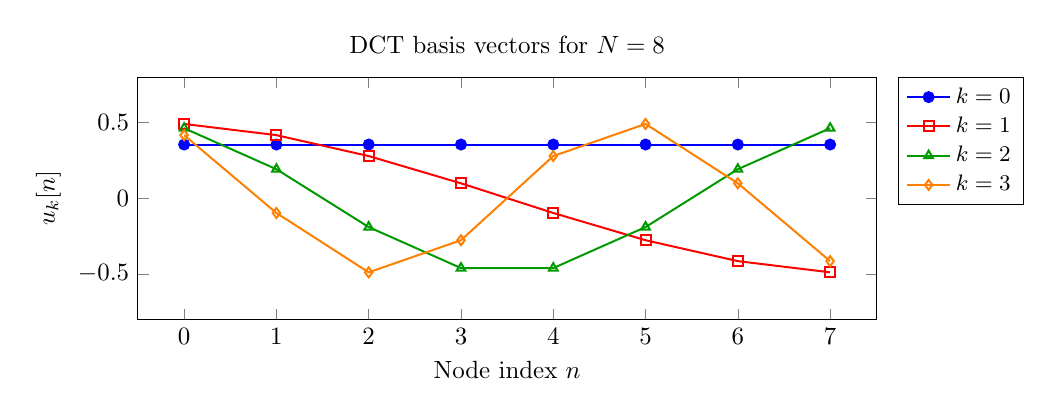
\begin{tikzpicture}[scale=0.9]
\begin{axis}[
    width=12cm, height=5cm,
    xlabel={Node index $n$},
    ylabel={$u_k[n]$},
    xmin=-0.5, xmax=7.5,
    ymin=-0.8, ymax=0.8,
    legend pos=outer north east,
    legend style={font=\small},
    title={DCT basis vectors for $N=8$}
]
% k=0 (constant)
\addplot[thick, blue, mark=*] coordinates {
    (0,0.354) (1,0.354) (2,0.354) (3,0.354) 
    (4,0.354) (5,0.354) (6,0.354) (7,0.354)
};
\addlegendentry{$k=0$}

% k=1
\addplot[thick, red, mark=square, mark size=2pt] coordinates {
    (0,0.490) (1,0.416) (2,0.278) (3,0.098) 
    (4,-0.098) (5,-0.278) (6,-0.416) (7,-0.490)
};
\addlegendentry{$k=1$}

% k=2
\addplot[thick, green!60!black, mark=triangle, mark size=2pt] coordinates {
    (0,0.462) (1,0.191) (2,-0.191) (3,-0.462) 
    (4,-0.462) (5,-0.191) (6,0.191) (7,0.462)
};
\addlegendentry{$k=2$}

% k=3
\addplot[thick, orange, mark=diamond, mark size=2pt] coordinates {
    (0,0.416) (1,-0.098) (2,-0.490) (3,-0.278) 
    (4,0.278) (5,0.490) (6,0.098) (7,-0.416)
};
\addlegendentry{$k=3$}
\end{axis}
\end{tikzpicture}
\caption{The first four DCT basis vectors for $N=8$. Compare with 
         Figure~3: same qualitative behavior (increasing oscillation 
         with $k$) but adapted to path boundary conditions.}
\end{figure}

%==========================================================================
\newpage
\section{Efficient Matrix Implementation for GPUs}
\label{dft-to-gnn:app:matrix-implementation}
%==========================================================================

The per-node message passing formulas are conceptually clear but 
computationally inefficient. For GPU acceleration, we must express 
everything as matrix operations. This appendix shows how.

\subsection{The Challenge}

Consider the GCN update for node $i$:
\[
h_i^{(l+1)} = \sigma\left( \sum_{j \in \mathcal{N}(i) \cup \{i\}} 
    \frac{1}{\sqrt{\hat{d}_i}\sqrt{\hat{d}_j}} h_j^{(l)} W^{(l)} \right)
\]

A naive implementation would loop over nodes and neighbors:
\begin{lstlisting}[style=pythonstyle, language=Python]
for i in range(N):
    h_new[i] = 0
    for j in neighbors[i] + [i]:
        h_new[i] += h[j] @ W / sqrt(d[i] * d[j])
    h_new[i] = relu(h_new[i])
\end{lstlisting}

This is $O(N \cdot \bar{d})$ sequential operations---very slow on GPUs, 
which excel at parallel matrix operations.

\subsection{Matrix Form of GCN}

The key insight is that the normalized adjacency matrix 
$\hat{P} = \hat{D}^{-1/2} \hat{A} \hat{D}^{-1/2}$ encodes all the 
neighborhood structure and normalization:
\[
\hat{P}_{ij} = \begin{cases}
\frac{1}{\sqrt{\hat{d}_i}\sqrt{\hat{d}_j}} & \text{if } j \in \mathcal{N}(i) \cup \{i\} \\
0 & \text{otherwise}
\end{cases}
\]

Then the entire GCN layer becomes:
\[
H^{(l+1)} = \sigma\left( \hat{P} \, H^{(l)} \, W^{(l)} \right)
\]

In code (PyTorch-style):
\begin{lstlisting}[style=pythonstyle, language=Python]
H_new = relu(P_hat @ H @ W)
\end{lstlisting}

This is just two matrix multiplications and an elementwise nonlinearity---highly 
optimized on GPUs.

\subsection{Sparse Matrix Operations}

For large graphs, $\hat{P}$ is sparse (most entries are zero). We store 
it in sparse format and use sparse-dense matrix multiplication:

\begin{lstlisting}[style=pythonstyle, language=Python]
# P_hat is sparse (N x N), H is dense (N x d), W is dense (d x d')
H_new = relu(sparse_mm(P_hat, H) @ W)
\end{lstlisting}

Complexity: $O(|E| \cdot d + N \cdot d \cdot d')$ instead of $O(N^2 \cdot d)$.

\subsection{Matrix Form of GAT}

GAT is trickier because attention weights depend on node features. The 
key steps are:

\textbf{Step 1: Compute all transformed features.}
\[
Z = H W \in \mathbb{R}^{N \times d'}
\]
where row $z_i = h_i W \in \mathbb{R}^{1 \times d'}$ is the transformed 
feature vector for node $i$.

\textbf{Step 2: Compute attention scores for all edges.}

For each edge $(i,j)$, we need to compute an attention score. Following 
the GAT formula, this involves:
\begin{itemize}
    \item $[z_i \| z_j]$: concatenation of the two row vectors, giving 
          a row vector in $\mathbb{R}^{1 \times 2d'}$
    \item $\mathbf{a} \in \mathbb{R}^{2d'}$: a learnable column vector
    \item $[z_i \| z_j] \, \mathbf{a}$: the dot product, giving a scalar
\end{itemize}

\textbf{The decomposition trick.} Naively computing $[z_i \| z_j]$ for 
all $|E|$ edges is expensive. Instead, we split $\mathbf{a}$ into two 
halves:
\[
\mathbf{a} = \begin{pmatrix} \mathbf{a}_1 \\ \mathbf{a}_2 \end{pmatrix}
\quad \text{where } \mathbf{a}_1, \mathbf{a}_2 \in \mathbb{R}^{d'}
\]

Then:
\[
[z_i \| z_j] \mathbf{a} = [z_i \| z_j] \begin{pmatrix} \mathbf{a}_1 \\ \mathbf{a}_2 \end{pmatrix}
= z_i \mathbf{a}_1 + z_j \mathbf{a}_2
\]

So we can precompute two vectors of size $N$ (one per node):
\begin{align*}
\mathbf{s}_1 &= Z \mathbf{a}_1 \in \mathbb{R}^{N} \quad \text{(score contribution from source node)} \\
\mathbf{s}_2 &= Z \mathbf{a}_2 \in \mathbb{R}^{N} \quad \text{(score contribution from target node)}
\end{align*}

The attention score for edge $(i,j)$ is then simply:
\[
e_{ij} = \text{LeakyReLU}(s_{1,i} + s_{2,j})
\]

This avoids forming $|E|$ concatenated vectors---we just index into two 
precomputed vectors of size $N$.

\textbf{Step 3: Compute attention scores for all edges.}

We compute $e_{ij}$ only for edges $(i,j) \in E$. Using the edge list:
\begin{lstlisting}[style=pythonstyle, language=Python]
# edge_index: (2, |E|) tensor of [source, target] indices
# edge_index[0] contains source nodes, edge_index[1] contains targets
e = leaky_relu(s1[edge_index[0]] + s2[edge_index[1]])  # shape: (|E|,)
\end{lstlisting}

\textbf{Step 4: Softmax per node.}

Apply softmax over each node's incoming edges (all edges with the same 
target node):
\begin{lstlisting}[style=pythonstyle, language=Python]
# For each target node, softmax over its incoming edges
alpha = sparse_softmax(e, index=edge_index[1], num_nodes=N)
\end{lstlisting}

\textbf{Step 5: Aggregate.}

Construct a sparse attention matrix $A_{\text{att}}$ where 
$(A_{\text{att}})_{ij} = \alpha_{ij}$ if $(i,j) \in E$ and $0$ otherwise. 
The final aggregation is:
\begin{lstlisting}[style=pythonstyle, language=Python]
# A_att: (N, N) sparse matrix with attention weights
H_new = sparse_mm(A_att, Z)  # shape: (N, d')
\end{lstlisting}

\subsection{General Message Passing in Matrix Form}

For a general message passing layer:
\[
h_i^{(l+1)} = \phi\left( h_i^{(l)}, \bigoplus_{j \in \mathcal{N}(i)} 
    \psi(h_i^{(l)}, h_j^{(l)}, e_{ij}) \right)
\]

The matrix implementation depends on the specific $\psi$ and $\bigoplus$:

\begin{center}
\renewcommand{\arraystretch}{1.3}
\begin{tabular}{lll}
\toprule
\textbf{Aggregation $\bigoplus$} & \textbf{Matrix Operation} & \textbf{Notes} \\
\midrule
Sum & $A \cdot H$ & Sparse matrix multiply \\
Mean & $D^{-1} A \cdot H$ & Row-normalized \\
Max & \texttt{scatter\_max} & Requires scatter ops \\
Attention & $\text{Softmax}(E) \cdot H$ & $E$ is score matrix \\
\bottomrule
\end{tabular}
\end{center}

\subsection{Example: Complete GCN Forward Pass}

\begin{example}[GCN in PyTorch]
Here is a complete GCN layer implementation:

\begin{lstlisting}[style=pythonstyle, language=Python]
import torch
import torch.nn as nn

class GCNLayer(nn.Module):
    def __init__(self, in_dim, out_dim):
        super().__init__()
        self.W = nn.Parameter(torch.randn(in_dim, out_dim))
        
    def forward(self, H, P_hat):
        """
        H: (N, in_dim) node features
        P_hat: (N, N) sparse normalized adjacency
        """
        # Aggregate then transform
        H_agg = torch.sparse.mm(P_hat, H)  # (N, in_dim)
        H_new = H_agg @ self.W              # (N, out_dim)
        return torch.relu(H_new)
\end{lstlisting}

The preprocessing (computing $\hat{P}$ from $A$) is done once:
\begin{lstlisting}[style=pythonstyle, language=Python]
def compute_P_hat(A, N):
    """A: (N, N) sparse adjacency matrix"""
    A_hat = A + torch.eye(N)           # Add self-loops
    D_hat = A_hat.sum(dim=1)           # Degrees
    D_inv_sqrt = D_hat.pow(-0.5)
    D_inv_sqrt[D_inv_sqrt == float('inf')] = 0
    # P_hat = D^{-1/2} A_hat D^{-1/2}
    P_hat = D_inv_sqrt.view(-1,1) * A_hat * D_inv_sqrt.view(1,-1)
    return P_hat.to_sparse()
\end{lstlisting}
\end{example}

\subsection{Batching Multiple Graphs}

For batching multiple graphs (common in graph classification), we 
create a block-diagonal adjacency matrix:

\[
A_{\text{batch}} = \begin{pmatrix}
A_1 & 0 & 0 \\
0 & A_2 & 0 \\
0 & 0 & A_3
\end{pmatrix}, \quad
H_{\text{batch}} = \begin{pmatrix}
H_1 \\ H_2 \\ H_3
\end{pmatrix}
\]

The same matrix operations work on the batched data, with no 
cross-graph message passing (ensured by the block structure).

%==========================================================================
\newpage
\begin{thebibliography}{99}

\bibitem{dft-to-gnn:bronstein2021geometric}
M.~M. Bronstein, J.~Bruna, T.~Cohen, and P.~Veličković.
\newblock Geometric Deep Learning: Grids, Groups, Graphs, Geodesics, and Gauges.
\newblock {\em arXiv preprint arXiv:2104.13478}, 2021.

\bibitem{dft-to-gnn:calder2025linear}
J.~Calder and P.~J. Olver.
\newblock {\em Linear Algebra, Data Science, and Machine Learning}.
\newblock 2025.

\bibitem{dft-to-gnn:kipf2017semi}
T.~N. Kipf and M.~Welling.
\newblock Semi-Supervised Classification with Graph Convolutional Networks.
\newblock In {\em International Conference on Learning Representations (ICLR)}, 2017.

\bibitem{dft-to-gnn:defferrard2016convolutional}
M.~Defferrard, X.~Bresson, and P.~Vandergheynst.
\newblock Convolutional Neural Networks on Graphs with Fast Localized Spectral Filtering.
\newblock In {\em Advances in Neural Information Processing Systems (NeurIPS)}, 2016.

\bibitem{dft-to-gnn:hamilton2017inductive}
W.~L. Hamilton, R.~Ying, and J.~Leskovec.
\newblock Inductive Representation Learning on Large Graphs.
\newblock In {\em Advances in Neural Information Processing Systems (NeurIPS)}, 2017.

\bibitem{dft-to-gnn:velickovic2018graph}
P.~Veličković, G.~Cucurull, A.~Casanova, A.~Romero, P.~Liò, and Y.~Bengio.
\newblock Graph Attention Networks.
\newblock In {\em International Conference on Learning Representations (ICLR)}, 2018.

\bibitem{dft-to-gnn:gilmer2017neural}
J.~Gilmer, S.~S. Schoenholz, P.~F. Riley, O.~Vinyals, and G.~E. Dahl.
\newblock Neural Message Passing for Quantum Chemistry.
\newblock In {\em International Conference on Machine Learning (ICML)}, 2017.

\bibitem{dft-to-gnn:shuman2013emerging}
D.~I. Shuman, S.~K. Narang, P.~Frossard, A.~Ortega, and P.~Vandergheynst.
\newblock The Emerging Field of Signal Processing on Graphs.
\newblock {\em IEEE Signal Processing Magazine}, 30(3):83--98, 2013.

\bibitem{dft-to-gnn:bruna2014spectral}
J.~Bruna, W.~Zaremba, A.~Szlam, and Y.~LeCun.
\newblock Spectral Networks and Locally Connected Networks on Graphs.
\newblock In {\em International Conference on Learning Representations (ICLR)}, 2014.

\bibitem{dft-to-gnn:wu2020comprehensive}
Z.~Wu, S.~Pan, F.~Chen, G.~Long, C.~Zhang, and P.~S. Yu.
\newblock A Comprehensive Survey on Graph Neural Networks.
\newblock {\em IEEE Transactions on Neural Networks and Learning Systems}, 32(1):4--24, 2020.

\bibitem{dft-to-gnn:chung1997spectral}
F.~R.~K. Chung.
\newblock {\em Spectral Graph Theory}.
\newblock American Mathematical Society, 1997.

\bibitem{dft-to-gnn:strang1999discrete}
G.~Strang.
\newblock The Discrete Cosine Transform.
\newblock {\em SIAM Review}, 41(1):135--147, 1999.

\end{thebibliography}
\end{notechapter}
